\documentclass[a4paper, titlepage, 12pt]{article}
\usepackage[left=3cm, right=3cm, top=3cm, bottom=3cm]{geometry}
\usepackage[utf8]{inputenc}
\usepackage[T1]{fontenc}
\usepackage[toc,titletoc,title]{appendix}
\usepackage{booktabs}
\usepackage{amsmath}
\usepackage{amssymb}
\usepackage{derivative}
% \usepackage{mathptmx} % Not sure if I like this font.
\usepackage{setspace}
\usepackage{color}
\usepackage{soul}
\usepackage{enumitem}
\usepackage{array}
\usepackage[hidelinks]{hyperref}
\usepackage{adjustbox}

% Graphics and TikZ stuff
\usepackage{graphicx}
\usepackage{tikz}
\usetikzlibrary{arrows}
\usetikzlibrary{arrows.meta,positioning}
\usepackage{caption}
\usepackage{subcaption}
\usetikzlibrary{calc}
\usepackage{blindtext}
\usetikzlibrary{intersections}
\tikzset{>=latex} % for LaTeX arrow head
\tikzstyle{curve}=[very thick,line cap=round]
% \tikzstyle{dashed curve}=[curve,thick,dashed]
\pgfdeclarelayer{back} % to draw on background
\pgfsetlayers{back,main} % set order
\usepackage{ifthen}
\usetikzlibrary{shapes.geometric}

% Caption setup
\captionsetup[figure]{font=small, labelfont=bf, labelsep=period}
\captionsetup[table]{font=small, labelfont=bf, labelsep=period}
\newcommand{\bcaption}[2]{\caption{\textbf{#1} #2}}

% Custom colours for diagrams etc.
\definecolor{s-color}{HTML}{41949A}
\definecolor{i-color}{HTML}{E56E5A}
\definecolor{r-color}{HTML}{7384BB}

% Prefer roman numeral subfigures
\renewcommand\thesubfigure{\roman{subfigure}}

% Fix todo notes / annotation margins
\setlength {\marginparwidth }{2cm}
% \usepackage[textwidth=2.5cm]{todonotes}
\usepackage[textwidth=2.5cm,disable]{todonotes}

% The following means texcount won't count the words in todonotes.
%TC:macro \todo 1
%TC:macro \hlnote 2

% This redefines the \todo command to always have small text and 0.5 spacing
\makeatletter
\renewcommand{\todo}[2][]{%
    \@todo[size=small, caption={#2}, #1]{\begin{spacing}{0.5}#2\end{spacing}}%
} 
\makeatother 

% This makes it so I can highlight specific words with notes
\makeatletter
 \if@todonotes@disabled
 \newcommand{\hlnote}[2]{#1}
 \else
 \newcommand{\hlnote}[2]{\todo{#2}\texthl{#1}}
 \fi
\makeatother

% Some bibliography configuration
% \usepackage[numbers,compress,sort]{natbib}
% \newcommand\newcite{\citet}	% to get "Author (Year)" with natbib
\usepackage[bibstyle=ieee, citestyle=numeric-comp, url=false]{biblatex}
% \usepackage[style=ieee, citecounter=true]{biblatex}
\newcommand{\citet}{\textcite}
\addbibresource{refs.bib} 
\renewcommand*{\bibfont}{\small}

% \renewcommand{\finentrypunct}{%
%   \addperiod\space
%   (Cited \arabic{citecounter}~time\ifnumequal{\value{citecounter}}{1}{}{s})%
% }

% Using microtype for better formatting, apparently
\AtBeginEnvironment{quote}{\par\singlespacing\small}
\usepackage{microtype}

% Macro to define quotations
\newcommand{\q}[1]{``#1''}

% Document information
\newcommand{\thesisTitle}{Simulating the Effects of Risk Perception and Human Behaviour on a Vector-borne Disease with Agent-based Modelling}

\newcommand{\name}{Jack Oliver}

\newcommand{\timeFrame}{School of Computing and Information Systems}

\newcommand{\school}{The University of Melbourne}

\newcommand{\supervisor}{Associate Professor Nic Geard}

\newcommand{\advisor}{Dr Cameron Zachreson}

\newcommand{\wordcount}{6,088}


% \setlength{\bibsep}{0.0pt}

% For presenting the RQs nicely
\newlist{questions}{enumerate}{2}
\setlist[questions,1]{label=\textbf{RQ\arabic*.},ref=\textbf{RQ\arabic*}}
\setlist[questions,2]{label=(\alph*),ref=\thequestionsi(\alph*)}

% Bibliography style - can change in the future.
% \bibliographystyle{agu}

% Using double spacing throughout proposal.
\doublespacing

\begin{document}

%TC:ignore
\begin{singlespace} % Single-space for the cover page
\begin{titlepage}
\begin{center}

% ------------------------------------------------------------
% TITLE PAGE
% ------------------------------------------------------------


\vspace*{1.5cm}

\Large{\textbf{\thesisTitle}}

\vspace{2.5cm}

\large{\textbf{\name} (1389498) \\ Length: {\wordcount} words} \\
\vspace{2cm}
\large{A research proposal submitted for the Master of Computer Science minor thesis component \\}
\vspace{.5cm}
\large{in the} \\
\large{\timeFrame} \\ 
\large{\textbf{\school}}

\vspace{2cm}

\large{\textbf{Primary Supervisor}}\\
\supervisor\\
\vspace{1.5cm}

\textbf{Co-Supervisor}\\
\advisor\\
\end{center}
\end{titlepage}
\end{singlespace}

\begin{spacing}{1.5}
    \tableofcontents
\end{spacing}
\clearpage

% ------------------------------------------------------------
% CONTENT
% ------------------------------------------------------------

%TC:endignore
\section{Introduction}\label{sec:introduction}

%Vector-borne diseases (VBDs) such as malaria, dengue, and chikungunya are major public health concerns, representing approximately 17\% of all infectious diseases and causing over 700,000 deaths annually \cite{world_health_organisation_who_vector-borne_2020}.  While vector control methods such as mosquito repellents and insecticide-treated bed nets effectively reduce disease transmission, these methods rely primarily on self-participation and voluntary adoption, which are driven by individuals' perceived risk of infection and personal behavioural attitudes. Mathematical models have become increasingly popular to help health practitioners anticipate downward pressure on health infrastructure and guide policy decisions for outbreak responses \cite{reiner_systematic_2013}. However, these models assume homogeneity of populations and thus cannot incorporate heterogeneous human behavioural attitudes that influence participation in vector control. Individual- or agent-based modelling is a computational technique that simulates the individual components (\textit{agents}) of a system to generate complex phenomena indirectly \cite{epstein_growing_1996}, offering a solution for directly encoding human behaviour. Despite the existing success of agent-based models in VBD applications, however, there is a lack of research investigating the dynamics between VBD spread and behaviours towards the use of preventive vector control tools.

Vector-borne diseases (VBDs) such as malaria, dengue, and chikungunya are major public health concerns, representing approximately 17\% of all infectious diseases worldwide \cite{world_health_organisation_who_vector-borne_2020}. While preventive measures such as mosquito repellent and insecticide-treated bed nets can effectively reduce disease transmission, these methods rely primarily on self-participation, which is driven by individuals' perceived risk of infection and personal behavioural attitudes. Mathematical models have become increasingly popular to anticipate downward pressure on health infrastructure and guide policy decisions for outbreak responses \cite{reiner_systematic_2013}. However, these models assume homogeneous populations, and thus cannot incorporate heterogeneous human behavioural attitudes that influence preventive measure adoption. Agent-based models (ABMs) are computational tools that simulate the individual components (\textit{agents}) of a system to generate complex phenomena indirectly \cite{epstein_growing_1996}, offering a solution for directly encoding human behaviour. Despite the existing success of ABMs in VBD applications, however, most of these models neglect this component and instead opt for simple models of human behaviour. While there is a wealth of literature from psychology and sociology to inform mechanisms of behaviour change in ABMs, there remains a lack of research that investigates how computationally encoding conceptual theories of behaviour in such models can capture complex patterns of preventive measure adoption and VBD spread.%Overall, there is a lack of research that investigates whether drawing on theories of behaviour from psychology and sociology can inform mechanisms of decision-making in ABMs of VBDs, capture complex patterns of preventive measure adoption and disease spread.

With more than 80\% of the global population living in areas vulnerable to at least one VBD \cite{golding_integrating_2015}, these diseases are major threats to worldwide public health infrastructure. Not only do VBDs result in epidemics which place large burdens on health institutions, but they can also stunt the economic development of communities, disproportionately affecting poorer nations \cite{lum_cost_2009, degroote_interventions_2018}. To curb the spread of VBDs, health officials employ \textit{vector control} to limit disease transmission from arthropods (such as mosquitoes, sandflies, and ticks) to humans. These chemical and non-chemical interventions such as mosquito repellent, insecticide-treated bed nets, and long-sleeved clothing are the primary---and often \textit{only}---strategy for reducing VBD spread due to a lack of a vaccine or preventive drug \cite{wilson_importance_2020}.

Although modern-day vector control methods can effectively reduce disease transmission, they primarily rely on self-participation and voluntary adoption of preventive measures, which are influenced by individuals' perceived risk of infection and personal behavioural attitudes \cite{winch_effectiveness_1992, brewer_risk_2004, raude_public_2012, lopes-rafegas_contribution_2023}. Risk perception and \textit{preventive behaviours} (behaviours that involve the use of preventive measures) are often recognised as profoundly important for understanding VBD spread, yet remain an understudied area \cite{williams_role_2010}. With additional issues surrounding vector control such as rising mosquito resistance to insecticides \cite{chala_emerging_2021, hemingway_averting_2016}, labour and funding disputes \cite{winch_effectiveness_1992}, and insufficient coverage and access within communities \cite{okumu_what_2022}, understanding how to motivate at-risk populations to adopt vector control tools for protection is an important public health concern. \\

To help health practitioners address VBD spread, mathematical models have become increasingly popular to guide policy and interventions by modelling the interactions between vector and human populations. These are equation-based models (EBMs), which express the dynamics of systems holistically through relationships in system variables \cite{van_dyke_parunak_agent-based_1998}, and provide utility in their tractable specification and analytical nature. In such models, however, risk perception and preventive behaviours have historically been neglected, despite their significance. This is largely due to the assumption of EBMs that populations are homogeneous or \textit{well mixed}, meaning heterogeneous factors of systems cannot be readily incorporated \cite{perkins_heterogeneity_2013, hunter_comparison_2018}.

Alternative mathematical methods for modelling VBDs also exist, such as statistical or machine learning approaches. For example, \citet{aerts_understanding_2020} used structural equation modelling to estimate the association between individuals' risk perception of VBDs and their tendencies to protect themselves. \citet{pley_digital_2021} highlighted artificial intelligence techniques as promising tools for VBD surveillance systems due to their ability to ingest data quickly and accurately predict epidemic outbreaks. However, such approaches often focus solely on prediction and require large amounts of data to be feasible. In VBD contexts, this is not always the case, as the value of modelling often instead lies in the ability to explain why certain dynamics arise, to illuminate core interactions of at-risk populations, and to discover new questions about behaviours that evolve alongside disease spread \cite{epstein_why_2008, bruch_agent-based_2015}. Ultimately, VBD models require an appropriate mechanistic underpinning to sufficiently consider complex social, community, and contextual human actions \cite{funk_modelling_2010, bedson_review_2021}.

Agent-based modelling is a \textit{bottom-up} computational modelling technique that simulates the individual components (\textit{agents}) of a system to reproduce emergent behaviour through stochastic interactions \cite{epstein_growing_1996}. Simulating systems at the individual level means heterogeneous factors of agents---such as risk perception and behavioural attitudes---can be naturally incorporated within models. Additionally, due to their modular implementation, agent-based models (ABMs) allow practitioners to represent hypothetical interventions without overhauling model architecture, unlike EBMs \cite{axtell_agent-based_2022}. This capacity for \textit{in silico} experimentation is especially useful in the context of VBDs, where analysing hypothetical interventions or counterfactual scenarios can be difficult given the data available, or lack thereof. The flexible nature of ABMs has spawned a growing body of research using the approach to model VBD spread \cite{krzhizhanovskaya_agent-based_2020, selvaraj_vector_2020, manore_network-patch_2015, linard_multi-agent_2009, jacintho_agent-based_2010, perkins_agent-based_2019, mulyani_agent_2017, maneerat_spatial_2016} and study the effects of risk perception and preventive behaviours on various infectious diseases \cite{mao_modeling_2014, kandiah_empirical_2017, du_how_2021, tully_coevolution_2013, andrews_disease_2015}. \\

There is sparse research, however, that investigates how realistic representations of human behaviour can be integrated within ABMs to capture complex patterns of preventive behaviours and disease spread. While simple representations of behaviour have previously been implemented in ABMs to study the dynamics of self-protection alongside epidemics \cite{mao_modeling_2014, barbrook-johnson_uses_2017, du_how_2021, scheidegger_agent-based_2017, mateus_c_modeling_2021}, these models have historically used simple threshold models of behaviour inspired by rational choice theory \cite{bedson_review_2021, janssen_empirically_2006, verelst_behavioural_2016}. Theoretical behaviour change theories from psychology and sociology are rarely used to inform decision-making processes in ABMs \cite{weston_infection_2018}, and little attention has been paid to the differences between computational implementations of these theories.

This research gap is recognised in the field as a missed opportunity, since drawing upon the wealth of theoretical behaviour change literature can arguably incorporate more nuanced representations of decision-making \cite{weston_infection_2018, funk_modelling_2010}. A deeper understanding of how preventive behaviours evolve within at-risk individuals may also aid the design of health interventions, and thus warrants further research into the implementation and impacts of conceptual behaviour change theories in ABMs.

%Ultimately, if modellers wish to embed realistic decision-making processes into infectious disease models, further research into the implementation and effects of conceptual behaviour change theories is needed.

%If policymakers and health officials wish to understand the interactions between disease spread and preventive behaviours, further research into epidemiological models that embed psychologically grounded behavioural processes \hlnote{is necessary}{Potentially too strong---reword to \q{has merit} or \q{is valuable}?}.

%There is sparse research, however, that employs ABMs to investigate the psychological mechanisms of behaviour change toward preventive measures for infectious diseases. While \hlnote{theories of behaviour change}{Terminology is not quite right (\q{behavioural change theory} is proper), but does this matter for introduction?} from psychology such as the Health Belief Model \cite{becker_health_1974} and Protection Motivation Theory \cite{rogers_protection_1975} have previously been implemented in ABMs \cite{abdulkareem_intelligent_2018, abdulkareem_risk_2020, durham_incorporating_2012, karimi_effect_2015}, few research efforts have attempted to quantify the impacts of employing different behaviour change theories within epidemiological models, despite existing literature suggesting their importance \cite{scheidegger_agent-based_2017, mateus_c_modeling_2021}. If policymakers and health officials wish to understand the interactions between disease spread and preventive behaviours, further research into epidemiological models that embed psychologically grounded behavioural processes \hlnote{is necessary}{Potentially too strong---reword to \q{has merit} or \q{is valuable}?}.

%how CBIs affect the spread of VBDs alongside the adoption of preventive measures, despite the fact that active community engagement has been shown to be necessary for effective vector control campaigns \cite{winch_effectiveness_1992, rivera_adoption_2023}. Furthermore, while psychological behavioural theories of decision-making such as the Health Belief Model \cite{becker_health_1974} and Protection Motivation Theory \cite{rogers_protection_1975} have previously been implemented in ABMs to simulate preventive behaviours \cite{abdulkareem_intelligent_2018, abdulkareem_risk_2020}, the area remains understudied, especially in the context of VBDs. Lastly, few research efforts have investigated the impacts of using different behavioural theories on disease spread in models, despite existing literature suggesting the importance of incorporating decision-making processes in ABMs \cite{scheidegger_agent-based_2017, mateus_c_modeling_2021}.

%Although the field is still evolving, ABMs have become popular tools for infectious disease modelling in public health contexts where heterogeneity is important \cite{tracy_agent-based_2018}. There is a growing body of research around VBD modelling for various geographical and spatial regions \cite{krzhizhanovskaya_agent-based_2020, selvaraj_vector_2020, manore_network-patch_2015, linard_multi-agent_2009, jacintho_agent-based_2010, perkins_agent-based_2019, mulyani_agent_2017, maneerat_spatial_2016} and the effects of risk perception and preventive behaviours on other infectious diseases \cite{mao_modeling_2014, kandiah_empirical_2017, du_how_2021, tully_coevolution_2013, andrews_disease_2015}. There is sparse research, however, that investigates how CBIs affect the spread of VBDs alongside the adoption of preventive measures, despite the fact that active community engagement has been shown to be necessary for effective vector control campaigns \cite{winch_effectiveness_1992, rivera_adoption_2023}. Furthermore, while psychological behavioural theories of decision-making such as the Health Belief Model \cite{becker_health_1974} and Protection Motivation Theory \cite{rogers_protection_1975} have previously been implemented in ABMs to simulate preventive behaviours \cite{abdulkareem_intelligent_2018, abdulkareem_risk_2020}, the area remains understudied, especially in the context of VBDs. Lastly, few research efforts have investigated the impacts of using different behavioural theories on disease spread in models, despite existing literature suggesting the importance of incorporating decision-making processes in ABMs \cite{scheidegger_agent-based_2017, mateus_c_modeling_2021}.

%The over-reliance on vector control commodities combined with the historical failings of global health institutions to effectively respond to emerging diseases in a timely manner \cite{bardosh_addressing_2017} has, in recent years, motivated a community-oriented approach to VBD spread. Community-based interventions (CBIs) are targeted approaches to address the expansion and emergence of VBDs by emphasising the \q{needs and capacities of vulnerable population groups and local stakeholders} \cite{bardosh_addressing_2017}. Examples include community empowerment campaigns, ecosystem management projects, and waste management programs \cite{perez_realist_2021}.

%While CBIs can ultimately increase vector control efficacy and reduce VBD severity, they primarily rely on influencing community engagement and participation in preventive measures, which are influenced by individuals' behavioural attitudes and perceived risk of infection \cite{winch_effectiveness_1992, brewer_risk_2004, raude_public_2012, lopes-rafegas_contribution_2023}. Therefore, in order to effectively support self-protection against VBDs within at-risk communities, policymakers need to understand the interaction between disease spread, risk perception, and \textit{preventive behaviours}---behaviours that involve the use of preventive measures.


\clearpage
\subsection{Research aims, question, and objectives}\label{sec:research-aims}

The research gap in the literature outlined above---the understudied effects of extending representations of human behaviour in ABMs for VBDs---motivates the research aims of this project. Specifically, this project aims to use computational models to quantify and investigate how integrating behaviour change theories within ABMs influences the adoption of preventive measures, and consequently, VBD spread. To make progress towards these aims, I investigate the following research question:

\vspace{.5cm}
\noindent\textit{How does representing human behaviour in computational models of vector-borne disease spread impact simulated infection dynamics and the estimated efficacy of health interventions?}
\vspace{.5cm}

In particular, I investigate how incorporating complex dynamics of preventive behaviours into a general model of VBD spread influences the adoption of preventive measures, such as insecticide-treated bed nets. Additionally, I compare how different behaviour change theories can be computationally represented in such models, and what their similarities and differences are when used to simulate preventive behaviours. In addressing this research question, I contribute a methodological study to the field of VBD modelling and analyse the impacts of different behavioural theories that describe psychological processes of protection motivation.

Specifically, the research objectives I set out to achieve within this thesis are:

\begin{objectives}[itemindent=4em]

\item Extend an established ABM of a VBD outbreak with preventive measures and contextual information from survey data.\label{ro1}

\item Parameterise the ABM with empirical data to contextualise the model to a real-world scenario.\label{ro2}

\item Computationally encode two behaviour change theories as agent decision-making processes.\label{ro3}

\item Analyse and compare the impacts of different behaviour change theories on preventive behaviours and disease spread for VBDs.\label{ro4}

\item Simulate hypothetical scenarios for each behaviour change theory to quantify the differences in output of disease spread and protection dynamics.\label{ro5}

\end{objectives}

\clearpage
\subsection{Thesis structure}

The structure of this thesis is as follows:

\paragraph{Chapter~\ref{sec:lit_review}.} First, I provide a comprehensive background of VBDs, vector control tools, risk perception, and behavioural attitudes towards preventive measures. I broadly review mathematical and agent-based approaches to modelling VBD spread before discussing the current landscape of ABMs that integrate preventive behaviours.

\paragraph{Chapter~\ref{sec:baseline_model}.} Next, I introduce the existing ABM chosen as a baseline model to extend within this thesis. I then detail the process to replicate the model and validate my implementation by reproducing the results of the original authors.

\paragraph{Chapter~\ref{sec:extended_model}.} After defining the baseline model, I address Objectives~\ref{ro1} and \ref{ro2} by outlining the extensions made to the model and detailing the parameterisation process to recreate a real-world setting based on qualitative and quantitative survey data. I then examine the behaviour of this model by varying its parameters and observing the subsequent impacts on disease spread.

\paragraph{Chapter~\ref{sec:bcts}.} Using the extended model, I complete Objectives~\ref{ro3}--\ref{ro5} by implementing two behaviour change theories as computational decision-making processes. I simulate hypothetical scenarios and compare output across these theories to assess the impacts on preventive behaviours and disease spread. Lastly, I conduct experiments to quantify the sensitivity of the implemented theories to changes in their inputs.

\paragraph{Chapter~\ref{sec:discussion}.} Using the results from the three previous chapters, I synthesise my findings to answer the research question. I discuss the strengths and contributions of my research and I conclude by highlighting the limitations and potential directions for future work.

\paragraph{Chapter~\ref{sec:conclusion}.} Lastly, I summarise the main findings of this thesis and I explain how my results are relevant to the broader research landscape.
\clearpage


\section{Related work}

In this section, I review past and present literature relevant to this proposed project. First, I present an overview of VBDs in epidemiological and modelling contexts, and examine how risk perception and behaviour change theories from psychology influence preventive behaviours. Second, I cover traditional methods for VBD modelling and I motivate agent-based modelling, before concluding with recent approaches to representing human behaviour in ABMs.


\subsection{Vector-borne diseases}

VBDs are infectious diseases that are major burdens on public health systems, with over one billion infections every year and symptomatic cases regularly requiring hospitalisation \cite{world_health_organisation_who_global_2004}. VBDs are spread by \textit{vectors}, which are living organisms that enable human-human or animal-human transmission of infectious pathogens, with examples including malaria and dengue, transmitted by mosquitoes, and leishmaniasis, transmitted by sandflies \cite{world_health_organisation_who_vector-borne_2020}. Not only do these diseases put pressure on health systems, but they also increase health inequalities and hinder socioeconomic development in developing nations that have insufficient coverage of health services, or tropical climates where VBDs are more common \cite{campbell-lendrum_climate_2015}.

There are multiple determinants that affect how VBDs spread. As demonstrated in Figure~\ref{fig:transmission-diagram}, VBDs can have bidirectional infection mechanisms, in which the vector infects the susceptible host, and the host can subsequently infect an uninfected vector. These host-vector transmission dynamics can be impacted by weather effects such as temperature and humidity, which affect feeding behaviour, survival rates, and reproduction among mosquitoes \cite{campbell-lendrum_climate_2015}.  Additionally, climate effects such as precipitation, floods, and droughts can influence vector abundance, activity, and transmission seasonality \cite{woolhouse_early_2001}. Individuals' demographic and socioecological factors like age, housing conditions, working situation, and knowledge of health services can also influence risk of infection \cite{chala_emerging_2021, hasyim_social_2019}.

\begin{figure}[h]
\centering

\begin{tikzpicture}[node distance=1cm, auto,
                >=Latex, 
                every node/.append style={align=center, font=\small},
                int/.style={draw, thick}]

\newcommand{\drawagentat}[4]{
    \tikzset{shift={(#1,#2)}}
    
    \path[draw=black,fill=#3,miter limit=10.0,scale=#4] (1.6431, -0.2275).. controls (1.5055, -0.2275) and (1.3944, -0.3387) .. (1.3944, -0.4763).. controls (1.3944, -0.6138) and (1.5055, -0.725) .. (1.6431, -0.725).. controls (1.7806, -0.725) and (1.8918, -0.6138) .. (1.8918, -0.4763).. controls (1.8918, -0.3387) and (1.7806, -0.2275) .. (1.6431, -0.2275) -- cycle(1.3679, -0.7911).. controls (1.1906, -0.7911) and (1.0478, -0.934) .. (1.0478, -1.1113) -- (1.0478, -1.8838).. controls (1.0478, -1.9447) and (1.0954, -1.9923) .. (1.1562, -1.9923).. controls (1.2171, -1.9923) and (1.2647, -1.9447) .. (1.2647, -1.8838) -- (1.2647, -1.1853) -- (1.3203, -1.1853).. controls (1.3203, -1.1853) and (1.3203, -3.0057) .. (1.3203, -3.1247).. controls (1.3203, -3.2041) and (1.3864, -3.2703) .. (1.4658, -3.2703).. controls (1.5478, -3.2703) and (1.6113, -3.2041) .. (1.6113, -3.1247) -- (1.6113, -1.9976) -- (1.6722, -1.9976) -- (1.6722, -3.1247).. controls (1.6722, -3.2041) and (1.7383, -3.2703) .. (1.8177, -3.2703).. controls (1.8997, -3.2703) and (1.9632, -3.2041) .. (1.9632, -3.1247) -- (1.9632, -1.1853) -- (2.0188, -1.1853) -- (2.0188, -1.8838).. controls (2.0188, -1.9447) and (2.0664, -1.9923) .. (2.1273, -1.9923).. controls (2.1881, -1.9923) and (2.2357, -1.9447) .. (2.2357, -1.8838) -- (2.2357, -1.1086).. controls (2.2357, -0.9313) and (2.0902, -0.7885) .. (1.9156, -0.7885).. controls (1.9182, -0.7911) and (1.3679, -0.7911) .. (1.3679, -0.7911) -- cycle;

    \tikzset{shift={(-#1,-#2)}}
    }

\newcommand{\drawmosquitoat}[3]{
    \tikzset{shift={(#1,#2)}}

    \path[draw=black,fill=#3,miter limit=10.0,line width=0.0001cm,scale=.5] (1.5779, -0.1786).. controls (1.5669, -0.1812) and (1.5472, -0.1912) .. (1.5356, -0.1999).. controls (1.4706, -0.2489) and (1.4023, -0.3617) .. (1.3047, -0.5818) -- (1.2865, -0.6227) -- (1.2778, -0.6065).. controls (1.2549, -0.5642) and (1.2251, -0.5267) .. (1.1826, -0.4866).. controls (1.1259, -0.4332) and (1.1002, -0.4158) .. (1.0708, -0.411).. controls (1.0548, -0.4083) and (1.0384, -0.4131) .. (1.0244, -0.4245).. controls (1.0177, -0.4299) and (1.0057, -0.4453) .. (0.9996, -0.4566).. controls (0.9873, -0.4783) and (0.9739, -0.5204) .. (0.9651, -0.5645).. controls (0.9486, -0.6463) and (0.939, -0.7409) .. (0.9265, -0.9452).. controls (0.9241, -0.9832) and (0.9232, -1.1225) .. (0.925, -1.173).. controls (0.9279, -1.2566) and (0.9328, -1.3343) .. (0.9423, -1.4448).. controls (0.9449, -1.4755) and (0.9471, -1.5021) .. (0.9471, -1.5041).. controls (0.9471, -1.5074) and (0.9464, -1.508) .. (0.942, -1.5087).. controls (0.9095, -1.5139) and (0.8738, -1.5243) .. (0.8494, -1.5358).. controls (0.7839, -1.5665) and (0.7361, -1.6163) .. (0.715, -1.6761).. controls (0.711, -1.6871) and (0.7099, -1.6882) .. (0.7055, -1.6845).. controls (0.7007, -1.6805) and (0.6862, -1.6726) .. (0.676, -1.6685).. controls (0.5991, -1.6377) and (0.5126, -1.6836) .. (0.4672, -1.7791).. controls (0.4606, -1.7928) and (0.4511, -1.8196) .. (0.4474, -1.8343) -- (0.4459, -1.8401) -- (0.4319, -1.8353).. controls (0.3542, -1.8082) and (0.2813, -1.7632) .. (0.2143, -1.7006) -- (0.1987, -1.686) -- (0.1785, -1.7062) -- (0.1582, -1.7265) -- (0.1747, -1.7422).. controls (0.2473, -1.8116) and (0.3334, -1.8639) .. (0.423, -1.8932) -- (0.4392, -1.8984) -- (0.4399, -1.9033).. controls (0.4403, -1.906) and (0.4414, -1.9127) .. (0.4424, -1.9182).. controls (0.4433, -1.9237) and (0.4439, -1.9285) .. (0.4435, -1.9286).. controls (0.4419, -1.9296) and (0.4016, -1.9362) .. (0.3884, -1.9377).. controls (0.3537, -1.9416) and (0.2951, -1.9416) .. (0.2574, -1.9377).. controls (0.237, -1.9355) and (0.2109, -1.9312) .. (0.1889, -1.9267).. controls (0.1782, -1.9245) and (0.1692, -1.9231) .. (0.1686, -1.9237).. controls (0.1682, -1.9242) and (0.1652, -1.9357) .. (0.162, -1.9493).. controls (0.1587, -1.9629) and (0.1559, -1.975) .. (0.1556, -1.9762).. controls (0.155, -1.978) and (0.1585, -1.9793) .. (0.1747, -1.9827).. controls (0.243, -1.9975) and (0.3129, -2.0023) .. (0.3788, -1.9966).. controls (0.4038, -1.9944) and (0.4509, -1.9871) .. (0.4628, -1.9835).. controls (0.4646, -1.983) and (0.4661, -1.9846) .. (0.4684, -1.9894).. controls (0.4776, -2.0074) and (0.5007, -2.0393) .. (0.5224, -2.0641) -- (0.5364, -2.08) -- (0.4775, -2.5068).. controls (0.4113, -2.9862) and (0.4163, -2.9414) .. (0.4274, -2.9532).. controls (0.441, -2.9675) and (0.465, -2.964) .. (0.4732, -2.9464).. controls (0.4752, -2.9424) and (0.5019, -2.8017) .. (0.5545, -2.5211).. controls (0.5976, -2.2905) and (0.6332, -2.1008) .. (0.6336, -2.0995).. controls (0.6339, -2.0983) and (0.6395, -2.094) .. (0.6459, -2.09).. controls (0.6794, -2.0695) and (0.7143, -2.0409) .. (0.7365, -2.0158).. controls (0.7651, -1.9835) and (0.7814, -1.9521) .. (0.7869, -1.9195) -- (0.7886, -1.909) -- (0.7961, -1.9149).. controls (0.8149, -1.9296) and (0.8453, -1.9462) .. (0.8723, -1.9562).. controls (0.8863, -1.9614) and (0.9164, -1.9695) .. (0.9283, -1.9713).. controls (0.9319, -1.9718) and (0.9348, -1.9727) .. (0.9348, -1.9732).. controls (0.9348, -1.9737) and (0.8922, -1.9996) .. (0.8403, -2.0307) -- (0.7459, -2.0874) -- (0.7468, -2.0959).. controls (0.7474, -2.1006) and (0.7628, -2.2306) .. (0.781, -2.3846) -- (0.8142, -2.665) -- (0.7426, -2.7558).. controls (0.6836, -2.8308) and (0.6712, -2.8471) .. (0.6728, -2.8485).. controls (0.6799, -2.8551) and (0.7155, -2.882) .. (0.7165, -2.8814).. controls (0.7172, -2.881) and (0.753, -2.8359) .. (0.7961, -2.7812) -- (0.8745, -2.6817) -- (0.8414, -2.4034).. controls (0.8233, -2.2502) and (0.8083, -2.1234) .. (0.8081, -2.1213).. controls (0.8078, -2.1178) and (0.8129, -2.1145) .. (0.9173, -2.0519) -- (1.0268, -1.9861) -- (1.0268, -2.0117) -- (1.0268, -2.0372) -- (0.9308, -2.1333) -- (0.8348, -2.2294) -- (0.9377, -2.5005).. controls (1.0287, -2.7403) and (1.0405, -2.772) .. (1.0394, -2.7757).. controls (1.0387, -2.7779) and (1.0173, -2.8259) .. (0.9919, -2.882).. controls (0.9665, -2.9381) and (0.9459, -2.9843) .. (0.946, -2.9845).. controls (0.9482, -2.9866) and (0.9981, -3.0079) .. (0.9987, -3.0069).. controls (0.9992, -3.0062) and (1.0229, -2.9537) .. (1.0515, -2.8904) -- (1.1034, -2.7751) -- (1.0027, -2.5097) -- (0.9021, -2.2445) -- (0.9933, -2.1532) -- (1.0844, -2.0619) -- (1.0844, -2.0125) -- (1.0844, -1.9631) -- (1.0985, -1.9585).. controls (1.1268, -1.9493) and (1.1573, -1.9334) .. (1.1835, -1.9141).. controls (1.1983, -1.9031) and (1.2228, -1.8785) .. (1.2345, -1.8628).. controls (1.2452, -1.8483) and (1.2574, -1.8254) .. (1.2636, -1.8083) -- (1.2678, -1.7963) -- (1.2747, -1.8055).. controls (1.3045, -1.8462) and (1.3557, -1.8935) .. (1.4132, -1.933) -- (1.4268, -1.9425) -- (1.4434, -1.9809).. controls (1.5992, -2.3424) and (1.8249, -2.6913) .. (2.0853, -2.9734).. controls (2.1174, -3.0083) and (2.2421, -3.1347) .. (2.3751, -3.2675).. controls (2.4783, -3.3706) and (2.4786, -3.3707) .. (2.491, -3.3708).. controls (2.4986, -3.3708) and (2.5102, -3.3649) .. (2.5142, -3.3586).. controls (2.5196, -3.3503) and (2.5209, -3.3431) .. (2.5183, -3.3341).. controls (2.5161, -3.3262) and (2.5151, -3.3254) .. (2.3413, -3.1512).. controls (2.1781, -2.9877) and (2.1495, -2.9585) .. (2.1125, -2.9178).. controls (1.9152, -2.7011) and (1.7411, -2.4489) .. (1.5967, -2.1702).. controls (1.5676, -2.1139) and (1.5104, -1.9945) .. (1.5119, -1.993).. controls (1.5122, -1.9927) and (1.5242, -1.9983) .. (1.5389, -2.0055).. controls (1.5794, -2.025) and (1.6312, -2.0464) .. (1.6606, -2.0559) -- (1.6706, -2.059) -- (1.6876, -2.0888).. controls (1.7911, -2.2693) and (1.9248, -2.4309) .. (2.0646, -2.5443).. controls (2.145, -2.6096) and (2.2281, -2.6597) .. (2.3128, -2.6943).. controls (2.3221, -2.698) and (2.3299, -2.7009) .. (2.3301, -2.7007).. controls (2.3309, -2.6997) and (2.3494, -2.6494) .. (2.3494, -2.6483).. controls (2.3494, -2.6478) and (2.3405, -2.6436) .. (2.3295, -2.639).. controls (2.1491, -2.5639) and (1.9748, -2.4107) .. (1.8226, -2.1934).. controls (1.8011, -2.1629) and (1.7604, -2.1001) .. (1.7532, -2.0865) -- (1.7517, -2.0836) -- (1.765, -2.0869).. controls (1.8057, -2.0968) and (1.8595, -2.1058) .. (1.9026, -2.1101).. controls (1.9359, -2.1134) and (2.0011, -2.1134) .. (2.0296, -2.1101).. controls (2.1515, -2.0961) and (2.2196, -2.0457) .. (2.22, -1.9692).. controls (2.2201, -1.9444) and (2.2149, -1.9239) .. (2.2012, -1.8958).. controls (2.1855, -1.8637) and (2.1652, -1.8365) .. (2.1318, -1.8031).. controls (2.1074, -1.7787) and (2.0924, -1.7657) .. (2.0629, -1.7433).. controls (2.0249, -1.7146) and (1.9751, -1.6837) .. (1.9331, -1.6626).. controls (1.9261, -1.6591) and (1.9204, -1.6554) .. (1.9204, -1.6546).. controls (1.9204, -1.6536) and (1.9304, -1.6318) .. (1.9425, -1.606) -- (1.9646, -1.5589) -- (1.9888, -1.5908).. controls (2.1673, -1.8266) and (2.3523, -2.0214) .. (2.5062, -2.1353).. controls (2.5221, -2.1473) and (2.5168, -2.1389) .. (2.5695, -2.2321).. controls (2.6142, -2.3112) and (2.6394, -2.3502) .. (2.6764, -2.3985).. controls (2.7088, -2.4408) and (2.7379, -2.4732) .. (2.7784, -2.5118).. controls (2.8458, -2.5763) and (2.9168, -2.6241) .. (2.9957, -2.6582) -- (3.0138, -2.6662) -- (3.0143, -2.6711) -- (3.0147, -2.6762) -- (3.0255, -2.6762).. controls (3.0468, -2.6762) and (3.0565, -2.6721) .. (3.0623, -2.6606).. controls (3.0664, -2.6522) and (3.0675, -2.6444) .. (3.0655, -2.6368).. controls (3.0624, -2.6254) and (3.0553, -2.6205) .. (3.0255, -2.6083).. controls (3.004, -2.5995) and (2.9587, -2.5761) .. (2.9366, -2.5624).. controls (2.888, -2.5321) and (2.8475, -2.4997) .. (2.8023, -2.4545).. controls (2.7551, -2.4073) and (2.7194, -2.3634) .. (2.6797, -2.3037).. controls (2.6617, -2.2765) and (2.6256, -2.2163) .. (2.6267, -2.2152).. controls (2.627, -2.2149) and (2.6363, -2.2198) .. (2.6476, -2.2258).. controls (2.6897, -2.2486) and (2.7291, -2.2648) .. (2.7921, -2.285).. controls (2.9323, -2.3297) and (3.031, -2.3496) .. (3.1248, -2.3518) -- (3.1587, -2.3527) -- (3.1587, -2.3235) -- (3.1587, -2.2946) -- (3.1399, -2.2946).. controls (3.0497, -2.2945) and (2.9471, -2.2741) .. (2.804, -2.228).. controls (2.7448, -2.2089) and (2.723, -2.2004) .. (2.6837, -2.1805).. controls (2.6551, -2.1662) and (2.6186, -2.1444) .. (2.5875, -2.1231) -- (2.5648, -2.1078) -- (2.5567, -2.0938).. controls (2.4746, -1.9522) and (2.3375, -1.7313) .. (2.2032, -1.5251).. controls (2.1623, -1.4623) and (2.0375, -1.275) .. (2.0359, -1.2741).. controls (2.0352, -1.2736) and (2.0331, -1.2768) .. (2.0312, -1.2812).. controls (2.0293, -1.2855) and (2.011, -1.3244) .. (1.9907, -1.3677) -- (1.9538, -1.4462) -- (1.9303, -1.413).. controls (1.9031, -1.374) and (1.8711, -1.3265) .. (1.8489, -1.292).. controls (1.8335, -1.268) and (1.8333, -1.2676) .. (1.8317, -1.2715).. controls (1.8308, -1.2735) and (1.8043, -1.343) .. (1.7729, -1.4256).. controls (1.7413, -1.5083) and (1.7153, -1.5762) .. (1.7151, -1.5765).. controls (1.7147, -1.5769) and (1.7026, -1.5743) .. (1.688, -1.5707).. controls (1.5384, -1.5341) and (1.4055, -1.5338) .. (1.3192, -1.5702).. controls (1.2877, -1.5834) and (1.2631, -1.6018) .. (1.248, -1.6236) -- (1.2427, -1.6314) -- (1.235, -1.6201) -- (1.2275, -1.6085) -- (1.295, -1.5407).. controls (1.4109, -1.4246) and (1.4906, -1.3355) .. (1.5698, -1.234).. controls (1.7196, -1.0417) and (1.8035, -0.8709) .. (1.8263, -0.7117).. controls (1.8409, -0.6094) and (1.8294, -0.5137) .. (1.791, -0.4187).. controls (1.7723, -0.3727) and (1.7319, -0.2971) .. (1.7015, -0.2513).. controls (1.6742, -0.2102) and (1.6459, -0.1858) .. (1.6175, -0.1786).. controls (1.607, -0.176) and (1.589, -0.176) .. (1.5779, -0.1786) -- cycle(2.0642, -1.4188).. controls (2.1854, -1.6011) and (2.327, -1.8232) .. (2.4194, -1.9761) -- (2.4355, -2.0027) -- (2.4227, -1.9912).. controls (2.2985, -1.8785) and (2.162, -1.7246) .. (2.0231, -1.5404).. controls (2.0066, -1.5187) and (1.9932, -1.5003) .. (1.9932, -1.4996).. controls (1.9932, -1.4989) and (2.0028, -1.4779) .. (2.0146, -1.4528).. controls (2.0264, -1.4277) and (2.0379, -1.4031) .. (2.0401, -1.3983).. controls (2.0423, -1.3935) and (2.0447, -1.3901) .. (2.0452, -1.3908).. controls (2.0459, -1.3914) and (2.0544, -1.4041) .. (2.0642, -1.4188) -- cycle(1.8622, -1.4156).. controls (1.8703, -1.4275) and (1.8878, -1.4524) .. (1.9009, -1.4709).. controls (1.9141, -1.4895) and (1.925, -1.5052) .. (1.925, -1.5059).. controls (1.925, -1.5072) and (1.8687, -1.6284) .. (1.8673, -1.6302).. controls (1.8667, -1.6308) and (1.8636, -1.6297) .. (1.8346, -1.6178).. controls (1.8234, -1.6131) and (1.8048, -1.6063) .. (1.7934, -1.6024).. controls (1.7822, -1.5986) and (1.7723, -1.5949) .. (1.7716, -1.5943).. controls (1.7709, -1.5938) and (1.7851, -1.5548) .. (1.8031, -1.5077).. controls (1.8452, -1.3971) and (1.8464, -1.394) .. (1.847, -1.394).. controls (1.8473, -1.394) and (1.8541, -1.4038) .. (1.8622, -1.4156) -- cycle;

    \tikzset{shift={(-#1,-#2)}}
}

\node[] (u-v) at (0,0) {Uninfected\\vector};
\node[below right=2.5cm of u-v] (i-h) {Infected\\host};
\node[below left=2.5cm of i-h] (i-v) {Infected\\vector};
\node[below left=2.5cm of u-v] (u-h) {Uninfected\\host};

\coordinate[above=1.5cm of i-h] (i-h2);

\path[->,thick,bend left]
    (u-v) edge node[font=\footnotesize] {bites} (i-h2)
    (i-h) edge node[font=\footnotesize] {infects} (i-v)
    (i-v) edge node[font=\footnotesize] {bites} (u-h);
\path[->,thick] (u-h) edge node[font=\footnotesize] {becomes} (i-h);

\drawmosquitoat{-.7}{2.2}{s-color}
\drawmosquitoat{-.6}{-3.35}{i-color}
\drawagentat{2.95}{-.95}{i-color}{.4}
\drawagentat{-4.55}{-.95}{s-color}{.4}

\end{tikzpicture}

\bcaption{Human-vector disease transmission for dengue.}{Hosts are infected by infectious mosquitoes, and mosquitoes are infected by infectious hosts. Adapted from \citet{krzhizhanovskaya_agent-based_2020}.}
\label{fig:transmission-diagram}
\end{figure}

\subsubsection{Vector control methods}

Most determinants of disease transmission mentioned above can be addressed through interventions known collectively as vector control, which can be broadly classified into chemical- and non-chemical-based tools \cite{wilson_importance_2020}. For example, housing conditions that are situated close to vector breeding grounds can be treated by spraying insecticides indoors to repel mosquitoes, and long-sleeved clothing can reduce the risk of being bitten while working in harsh outdoor conditions. Until the use of the first residual insecticide dichlorodiphenyltrichloroethane (commonly known as DDT) in the 1940s, vector control was essentially synonymous with environmental management \cite{wilson_importance_2020}. Nowadays, however, most vector control methods are chemical practices, such as outdoor fogging or spraying, and insecticide-treated nets.

Despite recent advancements in vector control, limiting VBD spread is still an ongoing and challenging public health concern. Vector populations are undergoing expansion and re-emergence in many areas previously thought to be essentially eradicated of disease \cite{atkinson_global_2010}. Concurrently, vectors are becoming increasingly resistant to insecticides \cite{degroote_interventions_2018, hemingway_averting_2016}, challenging the reliance on modern-day vector control methods. While insecticide resistance is an important factor for vector control, insecticides are arguably just one component of disease control, and an over-allocation of resources toward solving insecticide resistance may detract from \q{other key factors such as \dots effectively engaging communities,} according to \citet{okumu_what_2022}. Indeed, the need for holistic strategies that engage relevant social stakeholders has been echoed by experts in the field, highlighting the need for community-based approaches for VBD control \cite{bardosh_addressing_2017}.

Community-based interventions (CBIs) are interventions that promote VBD control through communal events. CBIs cover a broad range of interventions from surveillance and risk mapping projects to clean-up programs and educational empowerment campaigns \cite{perez_realist_2021}. While CBIs have the potential to increase the rate of use and effectiveness of vector control commodities \cite{winch_effectiveness_1992}, they require timely deployment and careful consideration of a community's character.  For example, \citet{sulistyawati_dengue_2019} emphasise the need to implement \q{bottom-up} CBIs that consider community opinions about vector control, in addition to improving \q{people's knowledge and motivation to participate.} Similarly, \citet{tapia-conyer_community_2012} raise concerns about CBIs that are successful in the short-term but have waning participation in the long run, arguing that for CBI success, \q{long-term behavioural modifications at an individual level are imperative.} Furthermore, CBIs can be ineffective in communities with a lack of political authority, and in fragmented societies where community members have competing interests or a lack of trust \cite{khun_community_2008}. Evidently, the success of CBIs to encourage preventive behaviours is dependent on policymakers' understanding and planning around the behavioural aspect of the community in question.

\subsubsection{Risk perception and human behaviour}\label{sec:risk-perception}

The dynamics between risk perception and preventive behaviours are understudied relationships in infectious disease literature, despite being profoundly important for understanding disease spread, and consequently, ways of designing effective CBIs \cite{williams_role_2010}. In their seminal papers, Weinstein \textit{et al.} \cite{weinstein_correct_1993, weinstein_use_1998} formulate hypotheses for the interactions between risk perception and preventive behaviours, which were later formalised by \citet{brewer_risk_2004} into the following:

\begin{description}
\item[Accuracy hypothesis.] Perceptions of risk accurately reflect one's (lack of) preventive behaviours.
\item[Behaviour motivation hypothesis.] Risk perception causes preventive behaviours.
\item[Risk reappraisal hypothesis.] Preventive behaviours lower risk perception.
\end{description}

The causal directionalities of these hypotheses are demonstrated in Figure~\ref{fig:risk_hypotheses}.

\begin{figure}[h]
\centering

\begin{tikzpicture}[node distance=1cm, auto,
                >=Latex, 
                every node/.append style={align=center, font=\small},
                int/.style={draw, thick}]

\node (prt1) {\textbf{Perceived risk}\\at time $t$};
\node[right=5cm of prt1] (prt2) {\textbf{Perceived risk}\\at time $t+1$};
\node[below=3cm of prt1] (pbt1) {\textbf{Preventive}\\\textbf{behaviour}\\at time $t$};
\node[below=3cm of prt2] (pbt2) {\textbf{Preventive}\\\textbf{behaviour}\\at time $t+1$};

\path[->, very thick] (prt1) edge node {$+$} (prt2)
    (prt1) edge node {$+$} (pbt2)
    (pbt2) edge node [align=right,font=\itshape] {Risk\\reappraisal\\hypothesis} (prt2)
    (pbt1) edge[dashed] node {$+$} (pbt2);
\path[<->, very thick]
    (pbt2) edge[bend right, in=-120, out=-60] node {$-$} (prt2)
    (prt1) edge[dashed, bend right,left] node [align=right,font=\itshape] {Accuracy\\hypothesis} (pbt1);

\node[align=left,font=\itshape] at (1.8,-2.2) {Behaviour\\motivation\\hypothesis};
\node[align=left,font=\itshape] at (11, -2) {Accuracy\\hypothesis};
\node at (8.3, -2) {$-$};
\node at (-.45, -2) {$-$};

\end{tikzpicture}

\bcaption{Risk perception and behaviour hypotheses.}{Straight lines indicate causal relationships, curved lines are non-causal. Signs ($+$ or $-$) indicate positive and negative influences respectively---for example, the risk reappraisal hypothesis causes a reduction in risk perception at time $t+1$. The accuracy hypothesis postulates that higher levels of risk perception accompany lower rates of preventive behaviour, although this is non-causal. Dashed arrows are included for completeness but not described. Adapted from \citet{brewer_risk_2004}.}
\label{fig:risk_hypotheses}
\end{figure}

Although risk perception is often regarded as a salient factor influencing preventive behaviours, the empirical evidence for this relationship is mixed. On the one hand, many studies have provided evidence for the three hypotheses above \cite{brewer_risk_2004, lopes-rafegas_contribution_2023, aerts_understanding_2020, qin_exploring_2021}, and the effect of risk perception for many phenomena is commonly regarded as a significant force for motivating preventive behaviours. As \citet{tan_severe_2004} put it, \q{when people perceive a health problem as serious they will take some kind of action.} Conversely, some studies have failed to support the hypotheses, such as \citet{raude_understanding_2019} who contested the risk reappraisal hypothesis, noting it could not explain the behaviours observed in their longitudinal study of chikungunya spread. However, previous research into the driving factors of risk perception for VBDs has shown that the perceived mosquito prevalence, amount of mosquito bites on an individual, and previous days with rainfall are important indicators for individuals when estimating their risk of VBD infection \cite{raude_public_2012, lopes-rafegas_contribution_2023, constant_ecology_2020}. Furthermore, as \citet{qin_exploring_2021} and others note, the lack of empirical evidence for the linkage between risk perception and preventive behaviour may be attributable to the dominance of cross-sectional studies in VBD literature. This is because cross-sectional studies only sample a population at a single point in time, and are therefore problematic for demonstrating causality as no temporal sequence can be established. To conclude, while the above hypotheses have been evidenced by practitioners across multiple epidemiological domains, there is currently no consensus on a complete mechanistic explanation as to why people adopt preventive measures.

Psychological behaviour change theories are frameworks that can provide researchers with hypotheses for why individuals change their behaviour, and can be applied to preventive behaviours for disease spread. According to a 2024 review by \citet{vande_velde_integrated_2024}, there are 83 behaviour change theories across the behavioural and social sciences. The Health Belief Model (HBM) and Protection Motivation Theory (PMT) are two pervasive theoretical models often used in VBD studies due to their existing bodies of research and empirical support. Originally introduced in the 1950s by \citet{hochbaum_public_1958}, and later extended by \citet{becker_health_1974}, the HBM combines factors of individuals to predict why people will adopt preventive behaviours for illnesses. The framework is rooted in value-expectation theory and is based on the assumption that individuals value avoiding illness, and will practice preventive measures if they expect actions to prevent or alleviate disease \cite{champion_health_2015}. In a similar vein, PMT was introduced in the 1970s by \citet{rogers_protection_1975} and later updated \cite{rogers_cognitive_1983}. PMT formulates the intent to adopt preventive measures based on individuals' appraisals of fear---the model postulates that individuals assess the significance of a perceived threat (in this case, disease) and the available methods of coping with the threat (preventive measures) to determine the behaviour they are most inclined to perform \cite{norman_protection_2015}. The HBM and PMT are more similar than different in formation, although PMT's inclusion of some external factors in shaping behavioural intent arguably makes the framework less focused on the individual compared to the HBM.

While PMT and the HBM have been applied to VBD studies to identify endogenous and exogenous factors that motivate the adoption of preventive measures \cite{vande_velde_integrated_2024, vizanko_modeling_2024, donohoe_tick-borne_2018, ghahremani_effect_2014}, both frameworks have been criticised to varying degrees. For example, \citet{bunton_theories_1991} and others have noted that the HBM does not \q{incorporate the wider context in which social decision and actions are taken} \cite{williams_role_2010}. Similarly, PMT has been criticised for lacking a social risk component, despite multiple studies demonstrating the importance of social risk severity perceptions for predicting preventive behaviours in other health scenarios \cite{pechmann_what_2003} and in VBD epidemics \cite{lopes-rafegas_contribution_2023, vande_velde_integrated_2024}. Furthermore, both the HBM and PMT are formulated in terms of behavioural \textit{intention}, not behaviour, and do not explicitly address this disconnect from intent to realised behaviour.

To address the need for a comprehensive behaviour change theory, \citet{michie_behaviour_2011} developed the COM-B (Capability, Opportunity, Motivation, and Behaviour) model, noting that the HBM fails to \q{address the important roles of impulsivity, habit, self-control, associative learning, and emotional progressing.} The COM-B model, or simply \textit{COM-B}, requires individuals to possess the physical and physiological capability to participate, the social and physical opportunity, and the sufficient endogenous motivation to adopt a behaviour. Unlike the HBM and PMT, COM-B was designed from the ground up to include social and environmental factors that influence behaviour, and provide a framework for characterising and designing specific interventions.


\subsubsection{Modelling vector-borne diseases}\label{sec:model-vbds}

From the above discussion, vector control campaigns evidently present a complex challenge for public health practitioners: health officials must consider not only effective commodities to curb disease transmission, but also the intricate socioeconomic factors that influence human behaviour and community participation. Fortunately, mathematical models have emerged as useful tools to guide policy decisions and vector control interventions by modelling the interactions between vector and human populations. The majority of these are compartmental equation-based models (EBMs), typically defined by a system of ordinary differential equations (ODEs) that explicitly represent the population-level mechanisms of disease spread. The SIR (Susceptible, Infected, and Recovered) model is perhaps the most basic and well-known compartmental model in epidemiology, and is defined by the differential equations in Figure~\ref{fig:sir-eqs}, and diagrammatically represented in Figure~\ref{fig:sir-diagram}. In the compartmental SIR model, each compartment ($S$, $I$, or $R$) represents either the number or proportion of individuals in each state. In the latter case shown in Figure~\ref{fig:sir-fig}, the sum of compartments $S+I+R=1$, and the differential equations govern the flow between states: $\beta$ is the rate of transmission, and $1/\gamma$ is the average infectious period.

\begin{figure}[htbp]
     \centering
     \begin{subfigure}[b]{0.3\textwidth}
         \centering
         \begin{align*}
             \dot{S}&=-\beta S I \\
             \dot{I}&=\beta S I - \gamma I \\
             \dot{R}&=\gamma I
         \end{align*}
         \vspace{.5cm}
         \caption{}
         \label{fig:sir-eqs}
     \end{subfigure}%
     \hfill
     \begin{subfigure}[b]{0.3\textwidth}
         \centering
         \begin{tikzpicture}[node distance=1cm, auto,
                >=Latex, 
                every node/.append style={align=center},
                int/.style={draw, thick, minimum width=2cm,minimum height=.6cm,rounded corners}]
            
               \node [int, fill=s-color, text=white] (S)             {$S$};
               \node [int, below=of S, fill=i-color, text=white] (I) {$I$};
               \node [int, below=of I, fill=r-color, text=white] (R) {$R$};
               \coordinate[below=of I] (out);
               \path[->] (S) edge node {$\beta S I$} (I)
                         (I) edge node {$\gamma$} (out);
        \end{tikzpicture}%
        \vspace{.1cm}
         \caption{}
         \label{fig:sir-diagram}
     \end{subfigure}%
     \hfill
     \begin{subfigure}[b]{0.3\textwidth}
         \centering
         \begin{tikzpicture}[x=0.025cm,y=3cm]
      \def\xmax{130.0} % x axis maximum
      \def\ymax{1.025} % y axis maximum
      
      % CURVES
      \draw[very thick,s-color] plot[smooth] coordinates {
        (0.0, 0.998)
        (1.0, 0.9973276981931711)
        (2.0, 0.9964840728072826)
        (3.0, 0.9954259410355902)
        (4.0, 0.9940995088472758)
        (5.0, 0.9924379202498846)
        (6.0, 0.9903583301294537)
        (7.0, 0.9877584623411796)
        (8.0, 0.9845126449693982)
        (9.0, 0.9804673761499587)
        (10.0, 0.9754365737308862)
        (11.0, 0.9691968214949727)
        (12.0, 0.9614831599950985)
        (13.0, 0.9519862997172801)
        (14.0, 0.940352554204059)
        (15.0, 0.9261882782122965)
        (16.0, 0.9090710438495231)
        (17.0, 0.8885700212989189)
        (18.0, 0.8642777263133894)
        (19.0, 0.8358540642118198)
        (20.0, 0.8030810771908262)
        (21.0, 0.7659229280505638)
        (22.0, 0.7245810914666934)
        (23.0, 0.6795310390592031)
        (24.0, 0.6315262208094109)
        (25.0, 0.5815597728549975)
        (26.0, 0.530784287703032)
        (27.0, 0.480401961203948)
        (28.0, 0.4315470131997255)
        (29.0, 0.3851844173656373)
        (30.0, 0.34204311236478063)
        (31.0, 0.30259079319787735)
        (32.0, 0.26704619116159567)
        (33.0, 0.23541747963832935)
        (34.0, 0.20755337693627968)
        (35.0, 0.18319550431436243)
        (36.0, 0.16202449489961224)
        (37.0, 0.14369631108544192)
        (38.0, 0.12786819190459633)
        (39.0, 0.1142154240467327)
        (40.0, 0.10244085770765672)
        (41.0, 0.09227917117513319)
        (42.0, 0.08349762407542727)
        (43.0, 0.07589465262860504)
        (44.0, 0.06929728200938529)
        (45.0, 0.06355801522279642)
        (46.0, 0.058551620655525126)
        (47.0, 0.054172042625136994)
        (48.0, 0.050329592261200325)
        (49.0, 0.04694844269012026)
        (50.0, 0.043964461012344906)
        (51.0, 0.04132334644651637)
        (52.0, 0.038979052841522095)
        (53.0, 0.03689245949626464)
        (54.0, 0.03503025674479982)
        (55.0, 0.0333640148992419)
        (56.0, 0.03186940716069393)
        (57.0, 0.03052556194112793)
        (58.0, 0.029314522922940435)
        (59.0, 0.028220798717186017)
        (60.0, 0.027230986866564763)
        (61.0, 0.02633345947719667)
        (62.0, 0.025518099944165016)
        (63.0, 0.024776082010869227)
        (64.0, 0.024099684200702437)
        (65.0, 0.023482133047441546)
        (66.0, 0.022917471110447615)
        (67.0, 0.02240044496406817)
        (68.0, 0.021926410315262507)
        (69.0, 0.021491251208289104)
        (70.0, 0.02109131113702911)
        (71.0, 0.02072333416281497)
        (72.0, 0.0203844144502876)
        (73.0, 0.020071952916559888)
        (74.0, 0.019783619900088856)
        (75.0, 0.01951732294773462)
        (76.0, 0.019271178924476662)
        (77.0, 0.01904348983513639)
        (78.0, 0.01883272179724266)
        (79.0, 0.018637486725199447)
        (80.0, 0.018456526325907375)
        (81.0, 0.01828869811954071)
        (82.0, 0.01813296312543959)
        (83.0, 0.0179883750995347)
        (84.0, 0.017854070995352137)
        (85.0, 0.017729262582964676)
        (86.0, 0.017613229006327027)
        (87.0, 0.017505310212865357)
        (88.0, 0.017404901096874745)
        (89.0, 0.0173114462974976)
        (90.0, 0.017224435562151353)
        (91.0, 0.017143399595539257)
        (92.0, 0.01706790635057259)
        (93.0, 0.016997557715887304)
        (94.0, 0.016931986521943748)
        (95.0, 0.016870853839826203)
        (96.0, 0.016813846588184817)
        (97.0, 0.016760675318771994)
        (98.0, 0.016711072272525326)
        (99.0, 0.016664789559655245)
        (100.0, 0.016621597566351946)
        (101.0, 0.01658128346014513)
        (102.0, 0.01654364986963487)
        (103.0, 0.016508513649971912)
        (104.0, 0.01647570478322638)
        (105.0, 0.016445065355601956)
        (106.0, 0.016416448635980945)
        (107.0, 0.01638971822340957)
        (108.0, 0.01636474727181619)
        (109.0, 0.016341417776474017)
        (110.0, 0.01631961991911177)
        (111.0, 0.016299251466096593)
        (112.0, 0.01628021721595586)
        (113.0, 0.016262428496385112)
        (114.0, 0.01624580267822401)
        (115.0, 0.016230262760800425)
        (116.0, 0.016215736962871975)
        (117.0, 0.01620215835153872)
        (118.0, 0.016189464506740366)
        (119.0, 0.016177597205375163)
        (120.0, 0.016166502123166716)
        (121.0, 0.01615612857185693)
        (122.0, 0.01614642924562425)
        (123.0, 0.016137359984575585)
        (124.0, 0.016128879567973667)
        (125.0, 0.01612094950436089)
      } node[above right] at (20.0, 0.85) {$S$};
    
      \draw[very thick,i-color] plot[smooth] coordinates {
        (0.0, 0.002)
        (1.0, 0.0025118551142537743)
        (2.0, 0.0031539938777885444)
        (3.0, 0.0039591662695688465)
        (4.0, 0.004968118489808619)
        (5.0, 0.00623140960500875)
        (6.0, 0.007811562939418319)
        (7.0, 0.009785566255793595)
        (8.0, 0.012247703979930483)
        (9.0, 0.015312646690744908)
        (10.0, 0.019118631546431588)
        (11.0, 0.023830424406796634)
        (12.0, 0.029641548066158235)
        (13.0, 0.036774978103104934)
        (14.0, 0.04548115670733093)
        (15.0, 0.056031784071024576)
        (16.0, 0.06870752067429403)
        (17.0, 0.08377764007513508)
        (18.0, 0.10147010366212483)
        (19.0, 0.12193183146840725)
        (20.0, 0.14518140067848814)
        (21.0, 0.17105999575147074)
        (22.0, 0.19919043532171044)
        (23.0, 0.22895696958160838)
        (24.0, 0.259518106856763)
        (25.0, 0.28985938667094235)
        (26.0, 0.3188829532686558)
        (27.0, 0.3455194399114178)
        (28.0, 0.3688394565809396)
        (29.0, 0.3881415222032409)
        (30.0, 0.4030005812795563)
        (31.0, 0.4132730399035242)
        (32.0, 0.41906532352012577)
        (33.0, 0.42067946344958507)
        (34.0, 0.4185502560260349)
        (35.0, 0.41318559720843967)
        (36.0, 0.40511699252513234)
        (37.0, 0.39486293867085376)
        (38.0, 0.3829048359712472)
        (39.0, 0.3696734068745041)
        (40.0, 0.35554304142539545)
        (41.0, 0.34083158946059094)
        (42.0, 0.32580354734024025)
        (43.0, 0.31067510055440883)
        (44.0, 0.29561995717048395)
        (45.0, 0.28077527980532796)
        (46.0, 0.26624730330554247)
        (47.0, 0.25211645104600255)
        (48.0, 0.2384418197612011)
        (49.0, 0.22526506832660712)
        (50.0, 0.21261370867495347)
        (51.0, 0.20050387694464075)
        (52.0, 0.1889426384526646)
        (53.0, 0.17792989454199318)
        (54.0, 0.16745995095769076)
        (55.0, 0.1575228009041371)
        (56.0, 0.1481051718320928)
        (57.0, 0.13919137482870902)
        (58.0, 0.13076399175912412)
        (59.0, 0.12280442866621256)
        (60.0, 0.11529335930002195)
        (61.0, 0.10821107868483248)
        (62.0, 0.10153778306609723)
        (63.0, 0.09525378974173093)
        (64.0, 0.08933970751617225)
        (65.0, 0.08377656795680846)
        (66.0, 0.07854592336352069)
        (67.0, 0.07362991889742818)
        (68.0, 0.06901134319755721)
        (69.0, 0.06467366191877792)
        (70.0, 0.06060103750187934)
        (71.0, 0.056778337871093404)
        (72.0, 0.053191136511508266)
        (73.0, 0.04982570562316056)
        (74.0, 0.04666900390809084)
        (75.0, 0.04370866035237411)
        (76.0, 0.04093295490047132)
        (77.0, 0.03833079688115406)
        (78.0, 0.03589170191195289)
        (79.0, 0.033605767757493035)
        (80.0, 0.0314636496459622)
        (81.0, 0.029456535300379883)
        (82.0, 0.02757612011540257)
        (83.0, 0.025814582538337398)
        (84.0, 0.024164559970481298)
        (85.0, 0.022619125203910007)
        (86.0, 0.021171763595026684)
        (87.0, 0.01981635095076292)
        (88.0, 0.018547132265826043)
        (89.0, 0.017358701287442397)
        (90.0, 0.016245980943696357)
        (91.0, 0.015204204657283225)
        (92.0, 0.014228898518535435)
        (93.0, 0.013315864297351382)
        (94.0, 0.012461163329890494)
        (95.0, 0.011661101240363472)
        (96.0, 0.010912213393931912)
        (97.0, 0.0102112512067788)
        (98.0, 0.0095551691146386)
        (99.0, 0.008941112345388831)
        (100.0, 0.008366405291875594)
        (101.0, 0.007828540611958488)
        (102.0, 0.007325168898255837)
        (103.0, 0.00685408898038212)
        (104.0, 0.00641323876526587)
        (105.0, 0.00600068664013983)
        (106.0, 0.005614623366158602)
        (107.0, 0.00525335446207554)
        (108.0, 0.004915293041732614)
        (109.0, 0.004598953085528574)
        (110.0, 0.004302943118755094)
        (111.0, 0.004025960273615112)
        (112.0, 0.003766784714830889)
        (113.0, 0.003524274404150664)
        (114.0, 0.003297360197385097)
        (115.0, 0.00308504122679214)
        (116.0, 0.0028863805892277226)
        (117.0, 0.0027005012887202306)
        (118.0, 0.002526582425212876)
        (119.0, 0.0023638556598361343)
        (120.0, 0.002211601837857245)
        (121.0, 0.0020691478868978476)
        (122.0, 0.0019358638729487004)
        (123.0, 0.001811160237143461)
        (124.0, 0.0016944852515148568)
        (125.0, 0.0015853225676223741)
        } node[above right] at (45.0, 0.3) {$I$};
    
        \draw[very thick,r-color] plot[smooth] coordinates {
        (0.0, 0.0)
        (1.0, 0.00016044669257483907)
        (2.0, 0.00036193331492854905)
        (3.0, 0.0006148926948404921)
        (4.0, 0.0009323726629151103)
        (5.0, 0.001330670145106066)
        (6.0, 0.001830106931127467)
        (7.0, 0.002455971403026405)
        (8.0, 0.0032396510506710074)
        (9.0, 0.004219977159296082)
        (10.0, 0.005444794722681841)
        (11.0, 0.006972754098230427)
        (12.0, 0.00887529193874307)
        (13.0, 0.011238722179614701)
        (14.0, 0.014166289088609818)
        (15.0, 0.017779937716678768)
        (16.0, 0.022221435476182713)
        (17.0, 0.027652338625945735)
        (18.0, 0.034252170024485565)
        (19.0, 0.0422141043197727)
        (20.0, 0.05173752213068529)
        (21.0, 0.06301707619796504)
        (22.0, 0.07622847321159593)
        (23.0, 0.09151199135918818)
        (24.0, 0.10895567233382564)
        (25.0, 0.12858084047405985)
        (26.0, 0.1503327590283119)
        (27.0, 0.17407859888463387)
        (28.0, 0.1996135302193346)
        (29.0, 0.22667406043112157)
        (30.0, 0.2549563063556628)
        (31.0, 0.2841361668985982)
        (32.0, 0.31388848531827834)
        (33.0, 0.34390305691208545)
        (34.0, 0.3738963670376853)
        (35.0, 0.40361889847719784)
        (36.0, 0.4328585125752554)
        (37.0, 0.46144075024370435)
        (38.0, 0.48922697212415656)
        (39.0, 0.5161111690787633)
        (40.0, 0.542016100866948)
        (41.0, 0.566889239364276)
        (42.0, 0.5906988285843326)
        (43.0, 0.6134302468169863)
        (44.0, 0.635082760820131)
        (45.0, 0.6556667049718758)
        (46.0, 0.6752010760389326)
        (47.0, 0.6937115063288607)
        (48.0, 0.7112285879775989)
        (49.0, 0.7277864889832728)
        (50.0, 0.7434218303127018)
        (51.0, 0.7581727766088432)
        (52.0, 0.7720783087058135)
        (53.0, 0.7851776459617423)
        (54.0, 0.7975097922975096)
        (55.0, 0.8091131841966213)
        (56.0, 0.8200254210072134)
        (57.0, 0.8302830632301633)
        (58.0, 0.8399214853179355)
        (59.0, 0.8489747726166015)
        (60.0, 0.8574756538334134)
        (61.0, 0.865455461837971)
        (62.0, 0.8729441169897378)
        (63.0, 0.8799701282473998)
        (64.0, 0.8865606082831254)
        (65.0, 0.89274129899575)
        (66.0, 0.8985366055260318)
        (67.0, 0.9039696361385037)
        (68.0, 0.9090622464871803)
        (69.0, 0.913835086872933)
        (70.0, 0.9183076513610916)
        (71.0, 0.9224983279660917)
        (72.0, 0.9264244490382042)
        (73.0, 0.9301023414602796)
        (74.0, 0.9335473761918203)
        (75.0, 0.9367740166998912)
        (76.0, 0.939795866175052)
        (77.0, 0.9426257132837095)
        (78.0, 0.9452755762908044)
        (79.0, 0.9477567455173074)
        (80.0, 0.9500798240281304)
        (81.0, 0.9522547665800793)
        (82.0, 0.9542909167591578)
        (83.0, 0.9561970423621279)
        (84.0, 0.9579813690341665)
        (85.0, 0.9596516122131252)
        (86.0, 0.9612150073986462)
        (87.0, 0.9626783388363717)
        (88.0, 0.9640479666372991)
        (89.0, 0.9653298524150598)
        (90.0, 0.9665295834941521)
        (91.0, 0.9676523957471773)
        (92.0, 0.9687031951308919)
        (93.0, 0.9696865779867614)
        (94.0, 0.9706068501481657)
        (95.0, 0.9714680449198103)
        (96.0, 0.9722739400178834)
        (97.0, 0.9730280734744492)
        (98.0, 0.9737337586128361)
        (99.0, 0.9743940980949559)
        (100.0, 0.9750119971417724)
        (101.0, 0.9755901759278963)
        (102.0, 0.9761311812321092)
        (103.0, 0.9766373973696458)
        (104.0, 0.9771110564515075)
        (105.0, 0.977554248004258)
        (106.0, 0.9779689279978604)
        (107.0, 0.9783569273145148)
        (108.0, 0.9787199596864512)
        (109.0, 0.9790596291379974)
        (110.0, 0.9793774369621331)
        (111.0, 0.9796747882602882)
        (112.0, 0.9799529980692132)
        (113.0, 0.9802132970994641)
        (114.0, 0.9804568371243909)
        (115.0, 0.9806846960124074)
        (116.0, 0.9808978824479002)
        (117.0, 0.9810973403597408)
        (118.0, 0.9812839530680466)
        (119.0, 0.9814585471347885)
        (120.0, 0.981621896038976)
        (121.0, 0.9817747235412451)
        (122.0, 0.9819177068814269)
        (123.0, 0.9820514797782809)
        (124.0, 0.9821766351805113)
        (125.0, 0.9822937279280166)
        } node[above right] at (75.0, 0.775) {$R$};

        % AXES
      \draw[<->,thick]
        (\xmax,0) node[below left] {$t$}
        -| (0,\ymax) node[above left,rotate=90] {Proportion};
    \end{tikzpicture}%
    \vspace{.05cm}
         \caption{}
         \label{fig:sir-curve}
     \end{subfigure}%
        \bcaption{Compartmental SIR model.}{\textbf{(i)} System of differential equations representing changes in flows between compartments. \textbf{(ii)} Compartmental diagram representing flows between compartments. \textbf{(iii)} SIR dynamics over time for $\beta=0.3$ and $1/\gamma=14$.}
        \label{fig:sir-fig}
\end{figure}

Compartmental models that extend the classical SIR model have long been used in epidemiological and VBD contexts \cite{tang_review_2020}. In his review, \citet{cosner_models_2015} covered spatial and non-spatial EBMs for VBDs, noting that \q{even simple models can provide insights into how movement patterns can affect disease transmission.} More complex EBMs have incorporated vector control measures such as drugs and insecticide spraying to analyse the efficacy and timeliness of these interventions \cite{reiner_systematic_2013}. Despite the success of these models, however, they are limited in that populations are assumed to be homogeneous, meaning infection rates and other factors such as mosquito biting rates are constant, despite studies suggesting otherwise \cite{perkins_heterogeneity_2013}. During their review of 388 equation-based VBD models from 1970 to 2010, \citet{reiner_systematic_2013} noted that most modern VBD models focused solely on \q{basic transmission dynamics} closely resembling the original Ross-Macdonald malaria model \cite{ross_report_1908,macdonald_epidemiology_1957} and claimed the field could benefit from models that incorporate heterogeneous factors.

There have been research efforts to facilitate heterogeneity in EBMs, despite the assumption of homogeneous populations. For example, \citet{perkins_heterogeneity_2013} proposed a framework for heterogeneous biting, transmission thresholds, and spatial scales of transmission by creating multiple \q{patches} or a \textit{metapopulation} that represented groups of populations characterised by different systems of equations. \citet{suarez_generic_2020} also used a patch-based architecture to develop an EBM that incorporated varied risk perception and demand for mosquito control. Similarly, \citet{roosa_general_2022} combined a patch model with an extended compartmental SIR model to represent the adoption of preventive measures within an EBM. Ultimately, however, ODE models are inherently incompatible with heterogeneity---specifying the dynamics of disease spread and behaviour at the population level means heterogeneity can only be captured via patches, yet as \citet{bedson_review_2021} point out, \q{the history of major epidemics demonstrates that \textit{microscale interactions between individuals} [emphasis added] are important.}

% ABMs

\subsection{Agent-based modelling}

The inability of EBMs to incorporate heterogeneity at the individual level outlined above is one reason why modellers have recently turned to the use of agent-based models (ABMs). Contrary to the top-down specification EBMs require, ABMs define a population of decentralised, autonomous agents that interact with one another to reproduce or \q{grow} emergent phenomena \cite{epstein_growing_1996}. Unlike the fixed system structure of EBMs, ABMs typically consist of simple rules that can be readily changed to alter system mechanisms. This \textit{bottom-up} approach to modelling naturally allows for the heterogeneity and adaptation of agents \cite{axtell_agent-based_2022}, and greatly simplifies the representation of interventions or counterfactual scenarios \cite{van_dyke_parunak_agent-based_1998}. In the context of epidemiology, an ABM can thus \q{function as an \textit{in silico} laboratory} for health practitioners to simulate populations encoded with heterogeneous biological, spatial, and behavioural characteristics \cite{marshall_formalizing_2015}.

A corollary of the malleable structure of ABMs is that existing models can be easily extended by other practitioners with alternative goals. The discrete agent-based representation of the SIR model illustrated in Figure~\ref{sir-abm-diag} is one example: $N$ agents encoded with the SIR states randomly move within an $N_b\times N_b$ lattice. If an infected agent and a susceptible agent occupy the same cell in any given time step, the susceptible agent is infected with probability $\beta$. Similar to the equation-based form, after an average $1/\gamma$ time steps, infected agents recover. Since ABMs are stochastic, simulations are often repeated and results are averaged over multiple runs, as shown in Figure~\ref{fig:sir-abm-avg}. The simple SIR model has been extended by, e.g., \citet{paoluzzi_single-agent_2021}, who alter agent mobility to investigate the impacts of restrictions during the COVID-19 epidemic.

\begin{figure}[h]
\centering

\begin{tikzpicture}[scale=1.1]
    \def\ioffset{0.525} % x axis maximum
    \def\matsize{5}
    
    % Draw labels
    \foreach \i in {0,1}
        \path (\i+\ioffset,-1+\ioffset) node{\i} (-1+\ioffset,\i+\ioffset) node{\i};
    \path (2+\ioffset,-1+\ioffset) node{$\dots$} (-1+\ioffset,2+\ioffset) node[rotate=90] {$\dots$};
    \path (3+\ioffset,-1+\ioffset) node{$i$} (-1+\ioffset,3+\ioffset) node{$j$};
    \path (4+\ioffset,-1+\ioffset) node{$\dots$} (-1+\ioffset,4+\ioffset) node[rotate=90] {$\dots$};
    \path (\matsize+\ioffset,-1+\ioffset) node{$N_b$} (-1+\ioffset,\matsize+\ioffset) node{$N_b$};
      
    % Draw lattice rects
    \foreach \i in {0,...,\matsize}
        \foreach \j in {0,...,\matsize}{
            % Check if current cell is (1,2) or (3,4) and color green
            \ifthenelse{\(\i=0 \AND \j=0\) \OR \(\i=0 \AND \j=2\) \OR \(\i=0 \AND \j=3\) \OR \(\i=0 \AND \j=4\) \OR \(\i=1 \AND \j=0\) \OR \(\i=1 \AND \j=1\) \OR \(\i=1 \AND \j=2\) \OR \(\i=2 \AND \j=0\) \OR \(\i=2 \AND \j=1\) \OR \(\i=2 \AND \j=2\) \OR \(\i=2 \AND \j=4\) \OR \(\i=3 \AND \j=1\) \OR \(\i=3 \AND \j=3\) \OR \(\i=3 \AND \j=4\) \OR \(\i=4 \AND \j=0\) \OR \(\i=4 \AND \j=4\) \OR \(\i=4 \AND \j=5\) \OR \(\i=5 \AND \j=0\) \OR \(\i=5 \AND \j=3\) \OR \(\i=5 \AND \j=4\)}{
                \fill[s-color] (\i+0.1,\j+0.1) rectangle (\i+0.95,\j+0.95);
            }{}

            \ifthenelse{\(\i=3 \AND \j=0\) \OR \(\i=4 \AND \j=3\) \OR \(\i=4 \AND \j=2\) \OR \(\i=2 \AND \j=5\)}{
                \fill[i-color] (\i+0.1,\j+0.1) rectangle (\i+0.95,\j+0.95);
            }{}

            \ifthenelse{\(\i=1 \AND \j=5\) \OR \(\i=5 \AND \j=5\) \OR \(\i=4 \AND \j=1\)}{
                \fill[r-color] (\i+0.1,\j+0.1) rectangle (\i+0.95,\j+0.95);
            }{}

            
            \draw[thick] (\i+0.1,\j+0.1) rectangle (\i+0.95,\j+0.95);
        };

    % Draw agents
    % R agents
    % \node[person,shirt=r-color,scale=1.2] at (1.1+\ioffset,5.3+\ioffset) {};
    % \node[person,shirt=r-color,scale=1.2] at (1-.1+\ioffset,5+\ioffset) {};
    
    % S agents
    % \node[person,shirt=s-color,scale=1.2] at (1-.1+\ioffset,1-.1+\ioffset) {};
    
    % \node[person,shirt=s-color,scale=1.2] at (2.1+\ioffset,1.3+\ioffset) {};
    % \node[person,shirt=s-color,scale=1.2] at (2-.1+\ioffset,1+\ioffset) {};

    % I agents
    % \node[black,scale=1.1] at (3-.1+\ioffset,0.1+\ioffset) {\usymH{1F6B9}{.9cm}};
    % \node[i-color] at (3-.1+\ioffset,0.1+\ioffset) {\usymH{1F6B9}{.8cm}};
    % \node[i-color] at (3-.1+\ioffset,0.1+\ioffset) {};

    \node[isosceles triangle, isosceles triangle apex angle=90, fill=s-color, minimum size=.66cm, rotate=225] at (4.38,2.37) {};
    \draw[thick] (4+0.1,2+0.1) rectangle (4+0.95,2+0.95);

    \newcommand{\drawagent}[1]{
    \path[draw=black,fill=#1,miter limit=10.0,scale=.3] (1.6431, -0.2275).. controls (1.5055, -0.2275) and (1.3944, -0.3387) .. (1.3944, -0.4763).. controls (1.3944, -0.6138) and (1.5055, -0.725) .. (1.6431, -0.725).. controls (1.7806, -0.725) and (1.8918, -0.6138) .. (1.8918, -0.4763).. controls (1.8918, -0.3387) and (1.7806, -0.2275) .. (1.6431, -0.2275) -- cycle(1.3679, -0.7911).. controls (1.1906, -0.7911) and (1.0478, -0.934) .. (1.0478, -1.1113) -- (1.0478, -1.8838).. controls (1.0478, -1.9447) and (1.0954, -1.9923) .. (1.1562, -1.9923).. controls (1.2171, -1.9923) and (1.2647, -1.9447) .. (1.2647, -1.8838) -- (1.2647, -1.1853) -- (1.3203, -1.1853).. controls (1.3203, -1.1853) and (1.3203, -3.0057) .. (1.3203, -3.1247).. controls (1.3203, -3.2041) and (1.3864, -3.2703) .. (1.4658, -3.2703).. controls (1.5478, -3.2703) and (1.6113, -3.2041) .. (1.6113, -3.1247) -- (1.6113, -1.9976) -- (1.6722, -1.9976) -- (1.6722, -3.1247).. controls (1.6722, -3.2041) and (1.7383, -3.2703) .. (1.8177, -3.2703).. controls (1.8997, -3.2703) and (1.9632, -3.2041) .. (1.9632, -3.1247) -- (1.9632, -1.1853) -- (2.0188, -1.1853) -- (2.0188, -1.8838).. controls (2.0188, -1.9447) and (2.0664, -1.9923) .. (2.1273, -1.9923).. controls (2.1881, -1.9923) and (2.2357, -1.9447) .. (2.2357, -1.8838) -- (2.2357, -1.1086).. controls (2.2357, -0.9313) and (2.0902, -0.7885) .. (1.9156, -0.7885).. controls (1.9182, -0.7911) and (1.3679, -0.7911) .. (1.3679, -0.7911) -- cycle;
    }

    \newcommand{\drawagentat}[3]{
    \tikzset{shift={(#2,#3)}}
    
    \path[draw=black,fill=#1,miter limit=10.0,scale=.3] (1.6431, -0.2275).. controls (1.5055, -0.2275) and (1.3944, -0.3387) .. (1.3944, -0.4763).. controls (1.3944, -0.6138) and (1.5055, -0.725) .. (1.6431, -0.725).. controls (1.7806, -0.725) and (1.8918, -0.6138) .. (1.8918, -0.4763).. controls (1.8918, -0.3387) and (1.7806, -0.2275) .. (1.6431, -0.2275) -- cycle(1.3679, -0.7911).. controls (1.1906, -0.7911) and (1.0478, -0.934) .. (1.0478, -1.1113) -- (1.0478, -1.8838).. controls (1.0478, -1.9447) and (1.0954, -1.9923) .. (1.1562, -1.9923).. controls (1.2171, -1.9923) and (1.2647, -1.9447) .. (1.2647, -1.8838) -- (1.2647, -1.1853) -- (1.3203, -1.1853).. controls (1.3203, -1.1853) and (1.3203, -3.0057) .. (1.3203, -3.1247).. controls (1.3203, -3.2041) and (1.3864, -3.2703) .. (1.4658, -3.2703).. controls (1.5478, -3.2703) and (1.6113, -3.2041) .. (1.6113, -3.1247) -- (1.6113, -1.9976) -- (1.6722, -1.9976) -- (1.6722, -3.1247).. controls (1.6722, -3.2041) and (1.7383, -3.2703) .. (1.8177, -3.2703).. controls (1.8997, -3.2703) and (1.9632, -3.2041) .. (1.9632, -3.1247) -- (1.9632, -1.1853) -- (2.0188, -1.1853) -- (2.0188, -1.8838).. controls (2.0188, -1.9447) and (2.0664, -1.9923) .. (2.1273, -1.9923).. controls (2.1881, -1.9923) and (2.2357, -1.9447) .. (2.2357, -1.8838) -- (2.2357, -1.1086).. controls (2.2357, -0.9313) and (2.0902, -0.7885) .. (1.9156, -0.7885).. controls (1.9182, -0.7911) and (1.3679, -0.7911) .. (1.3679, -0.7911) -- cycle;

    \tikzset{shift={(-#2,-#3)}}
    }

    % S agents
    \tikzset{shift={(.4+\ioffset,1.7+\ioffset)}}
        \drawagent{s-color}
    \tikzset{shift={(1.25,.25)}}
        \drawagent{s-color}
    \tikzset{shift={(-.35,-.25)}}
        \drawagent{s-color}

    % R agents
    \tikzset{shift={(-.95,4.2)}}
        \drawagent{r-color}
    \tikzset{shift={(.3,-.1)}}
        \drawagent{r-color}
    \tikzset{shift={(-.2,-.15)}}
        \drawagent{r-color}

    % I agent
    \tikzset{shift={(1.85,-4.7)}}
        \drawagent{i-color}

    % S and I agent
    \tikzset{shift={(1.4,2.05)}}
        \drawagent{i-color}
    \tikzset{shift={(-.35,-.23)}}
        \drawagent{s-color}

    % Equations
    \tikzset{shift={(3.25, 1.8)}}
    \node[] at (0,0) {\textbf{(a)}};
    \drawagentat{s-color}{0.2}{-.1}
    \drawagentat{i-color}{0.6}{-.8}
    \path[->, draw, thick] (1.8, -1) -- (3, -1);
    \node at (2.4, -.7) {$\beta$};
    
    \drawagentat{i-color}{3.1}{-.1}
    \drawagentat{i-color}{3.5}{-.8}

    \tikzset{shift={(0, -3)}}
    \node[] at (0,0) {\textbf{(b)}};
    \drawagentat{i-color}{0.4}{-.1}
    \path[->, draw, thick] (1.6, -.5) -- (3, -.5);
    \node at (2.2, -.2) {$\gamma$};
    \drawagentat{r-color}{3.1}{-.1}
    
    
\end{tikzpicture}

\bcaption{Example ABM of SIR dynamics on a lattice.}{Agents with different SIR states move randomly from any cell to any orthogonally adjacent cell. Teal agents are susceptible, red agents are infected, and purple agents are recovered. Not all agents are shown. (Multi-)coloured cells correspond to the SIR state of agents within that cell, and white cells are unoccupied. \textbf{(a)} Susceptible agents that share a cell with infected agents are infected with probability $\beta$ during each time step. \textbf{(b)} Infected agents recover after an average $1/\gamma$ time steps. Adapted from \citet{paoluzzi_single-agent_2021}.}
\label{sir-abm-diag}
\end{figure}

\begin{figure}[htbp]
    \centering

    \begin{tikzpicture}[>=stealth]
    % LHS plot 1
    \draw[curve,s-color] plot[smooth] coordinates {
    (-8.0, 3.49)
    (-7.724024512482009, 3.3899999999999997)
    (-7.6484637396372115, 3.3200000000000003)
    (-7.575293451467849, 3.26)
    (-7.503363558513278, 3.17)
    (-7.431975571153575, 3.1)
    (-7.4034740477674585, 3.04)
    (-7.347587243310602, 2.9699999999999998)
    (-7.319165044453064, 2.92)
    (-7.295761688316618, 2.85)
    (-7.256915998988681, 2.79)
    (-7.227168918566119, 2.73)
    (-7.214826797701855, 2.6399999999999997)
    (-7.190112056349427, 2.56)
    (-7.145799388697578, 2.51)
    (-7.114025393756335, 2.43)
    (-7.083940841055886, 2.4)
    (-7.065913148865518, 2.34)
    (-7.040632834972005, 2.2800000000000002)
    (-7.020523178328933, 2.21)
    (-6.994840986408573, 2.13)
    (-6.964917234604183, 2.07)
    (-6.935920958726876, 2.01)
    (-6.90240456136456, 1.96)
    (-6.871291715913282, 1.92)
    (-6.8479224101567615, 1.87)
    (-6.818213573307265, 1.83)
    (-6.776110138898, 1.78)
    (-6.700132590103333, 1.75)
    (-6.658815900705981, 1.74)
    (-6.57460720665217, 1.7)
    (-6.529765752224526, 1.68)
    (-6.45546739165365, 1.67)
    (-6.410288267674974, 1.65)
    (-6.332084009436284, 1.62)
    (-6.292160628893704, 1.59)
    (-6.164451622325407, 1.57)
    (-5.948722216423396, 1.57)
    (-5.5, 1.57)
    };
    
    \draw[curve,i-color] plot[smooth] coordinates {
    (-8.0, 1.51)
    (-7.724024512482009, 1.61)
    (-7.6484637396372115, 1.65)
    (-7.575293451467849, 1.67)
    (-7.503363558513278, 1.75)
    (-7.431975571153575, 1.79)
    (-7.4034740477674585, 1.81)
    (-7.347587243310602, 1.85)
    (-7.319165044453064, 1.85)
    (-7.295761688316618, 1.8900000000000001)
    (-7.256915998988681, 1.91)
    (-7.227168918566119, 1.93)
    (-7.214826797701855, 2.01)
    (-7.190112056349427, 2.07)
    (-7.145799388697578, 2.07)
    (-7.114025393756335, 2.13)
    (-7.083940841055886, 2.09)
    (-7.065913148865518, 2.11)
    (-7.040632834972005, 2.13)
    (-7.020523178328933, 2.17)
    (-6.994840986408573, 2.23)
    (-6.964917234604183, 2.25)
    (-6.935920958726876, 2.27)
    (-6.90240456136456, 2.27)
    (-6.871291715913282, 2.25)
    (-6.8479224101567615, 2.25)
    (-6.818213573307265, 2.23)
    (-6.776110138898, 2.23)
    (-6.700132590103333, 2.19)
    (-6.658815900705981, 2.11)
    (-6.57460720665217, 2.09)
    (-6.529765752224526, 2.0300000000000002)
    (-6.45546739165365, 1.95)
    (-6.410288267674974, 1.8900000000000001)
    (-6.332084009436284, 1.85)
    (-6.292160628893704, 1.81)
    (-6.164451622325407, 1.75)
    (-5.948722216423396, 1.65)
    (-5.5, 1.55)
    };
    
    \draw[curve,r-color] plot[smooth] coordinates {
    (-8.0, 1.5)
    (-7.724024512482009, 1.5)
    (-7.6484637396372115, 1.53)
    (-7.575293451467849, 1.57)
    (-7.503363558513278, 1.58)
    (-7.431975571153575, 1.61)
    (-7.4034740477674585, 1.65)
    (-7.347587243310602, 1.68)
    (-7.319165044453064, 1.73)
    (-7.295761688316618, 1.76)
    (-7.256915998988681, 1.8)
    (-7.227168918566119, 1.84)
    (-7.214826797701855, 1.85)
    (-7.190112056349427, 1.87)
    (-7.145799388697578, 1.92)
    (-7.114025393756335, 1.94)
    (-7.083940841055886, 2.01)
    (-7.065913148865518, 2.05)
    (-7.040632834972005, 2.09)
    (-7.020523178328933, 2.12)
    (-6.994840986408573, 2.14)
    (-6.964917234604183, 2.18)
    (-6.935920958726876, 2.2199999999999998)
    (-6.90240456136456, 2.27)
    (-6.871291715913282, 2.33)
    (-6.8479224101567615, 2.38)
    (-6.818213573307265, 2.44)
    (-6.776110138898, 2.49)
    (-6.700132590103333, 2.56)
    (-6.658815900705981, 2.65)
    (-6.57460720665217, 2.71)
    (-6.529765752224526, 2.79)
    (-6.45546739165365, 2.88)
    (-6.410288267674974, 2.96)
    (-6.332084009436284, 3.0300000000000002)
    (-6.292160628893704, 3.1)
    (-6.164451622325407, 3.1799999999999997)
    (-5.948722216423396, 3.2800000000000002)
    (-5.5, 3.38)
    };
    \draw[->,thick] (-8, 1.5) -- (-5.5, 1.5) node[below left] {$t$};
    \draw[->,thick] (-8, 1.5) -- (-8, 3.5) node[left] {$N$};

    % Dots sep
    \node[rotate=90] at (-7, 0.5) {$\dots$};

    % LHS plot 2
    \draw[curve,s-color] plot[smooth] coordinates {
    (-8.0, -0.010000000000000009)
    (-7.675905625901207, -0.10000000000000009)
    (-7.621177873639785, -0.1399999999999999)
    (-7.489215140697653, -0.17999999999999994)
    (-7.313191941569358, -0.26)
    (-7.265868612764226, -0.3500000000000001)
    (-7.2125195166257425, -0.41999999999999993)
    (-7.178492874106199, -0.47)
    (-7.1128509571699565, -0.54)
    (-7.056309963409815, -0.6100000000000001)
    (-7.026302877482503, -0.6799999999999999)
    (-7.007564697872866, -0.74)
    (-6.98289200110431, -0.81)
    (-6.9625713352402165, -0.8899999999999999)
    (-6.942163035482007, -0.97)
    (-6.9188938759677345, -1.01)
    (-6.90205091717434, -1.08)
    (-6.882410313609648, -1.13)
    (-6.82859443430481, -1.19)
    (-6.808009913481963, -1.25)
    (-6.789774262276251, -1.3199999999999998)
    (-6.7655252416613365, -1.3900000000000001)
    (-6.749582998055055, -1.4300000000000002)
    (-6.694128785342196, -1.48)
    (-6.656313058529874, -1.51)
    (-6.636879919955421, -1.52)
    (-6.597415012880587, -1.56)
    (-6.576119689438654, -1.58)
    (-6.536477553994184, -1.6099999999999999)
    (-6.492760121430862, -1.67)
    (-6.441313105638984, -1.68)
    (-6.381648323533211, -1.69)
    (-6.28967941046716, -1.69)
    (-6.160565722289649, -1.72)
    (-5.901152655592379, -1.75)
    (-5.5, -1.77)
    };
    
    \draw[curve,i-color] plot[smooth] coordinates {
    (-8.0, -1.99)
    (-7.675905625901207, -1.91)
    (-7.621177873639785, -1.93)
    (-7.489215140697653, -1.95)
    (-7.313191941569358, -1.89)
    (-7.265868612764226, -1.81)
    (-7.2125195166257425, -1.77)
    (-7.178492874106199, -1.77)
    (-7.1128509571699565, -1.73)
    (-7.056309963409815, -1.69)
    (-7.026302877482503, -1.65)
    (-7.007564697872866, -1.63)
    (-6.98289200110431, -1.59)
    (-6.9625713352402165, -1.53)
    (-6.942163035482007, -1.47)
    (-6.9188938759677345, -1.49)
    (-6.90205091717434, -1.45)
    (-6.882410313609648, -1.45)
    (-6.82859443430481, -1.4300000000000002)
    (-6.808009913481963, -1.4100000000000001)
    (-6.789774262276251, -1.37)
    (-6.7655252416613365, -1.33)
    (-6.749582998055055, -1.35)
    (-6.694128785342196, -1.35)
    (-6.656313058529874, -1.3900000000000001)
    (-6.636879919955421, -1.47)
    (-6.597415012880587, -1.49)
    (-6.576119689438654, -1.55)
    (-6.536477553994184, -1.59)
    (-6.492760121430862, -1.57)
    (-6.441313105638984, -1.65)
    (-6.381648323533211, -1.73)
    (-6.28967941046716, -1.83)
    (-6.160565722289649, -1.87)
    (-5.901152655592379, -1.91)
    (-5.5, -1.97)
    };
    
    \draw[curve,r-color] plot[smooth] coordinates {
    (-8.0, -2.0)
    (-7.675905625901207, -1.99)
    (-7.621177873639785, -1.93)
    (-7.489215140697653, -1.87)
    (-7.313191941569358, -1.85)
    (-7.265868612764226, -1.84)
    (-7.2125195166257425, -1.81)
    (-7.178492874106199, -1.76)
    (-7.1128509571699565, -1.73)
    (-7.056309963409815, -1.7)
    (-7.026302877482503, -1.67)
    (-7.007564697872866, -1.63)
    (-6.98289200110431, -1.6)
    (-6.9625713352402165, -1.58)
    (-6.942163035482007, -1.56)
    (-6.9188938759677345, -1.5)
    (-6.90205091717434, -1.47)
    (-6.882410313609648, -1.42)
    (-6.82859443430481, -1.38)
    (-6.808009913481963, -1.3399999999999999)
    (-6.789774262276251, -1.31)
    (-6.7655252416613365, -1.28)
    (-6.749582998055055, -1.22)
    (-6.694128785342196, -1.17)
    (-6.656313058529874, -1.1)
    (-6.636879919955421, -1.01)
    (-6.597415012880587, -0.95)
    (-6.576119689438654, -0.8700000000000001)
    (-6.536477553994184, -0.8)
    (-6.492760121430862, -0.76)
    (-6.441313105638984, -0.6699999999999999)
    (-6.381648323533211, -0.5800000000000001)
    (-6.28967941046716, -0.48)
    (-6.160565722289649, -0.4099999999999999)
    (-5.901152655592379, -0.3400000000000001)
    (-5.5, -0.26)
    };
    \draw[->,thick] (-8, -2) -- (-5.5, -2) node[below left] {$t$};
    \draw[->,thick] (-8, -2) -- (-8, 0) node[left] {$N$};

    % Right side plot

    \newcommand{\xshift}{-.65}
  \newcommand{\yshift}{-.5}
  \newcommand{\newyscale}{.3}
  \newcommand{\newxscale}{.25}

  % \scalebox{.25}[.3]{

  \tikzset{shift={(\xshift,\yshift)}}

  \begin{scope}[line cap=butt,line join=round,xscale=\newxscale,yscale=\newyscale]
    \begin{scope}[line cap=butt,line join=round]
      \path[fill=white,line cap=butt,line join=round] (0.0, 0.0) -- (16.256, 0.0) -- (16.256, 12.192) -- (0.0, 12.192) -- cycle;



    \end{scope}
    \begin{scope}[line cap=butt,line join=round]
      \begin{scope}[line cap=butt,line join=round]
        \begin{scope}[line cap=butt,line join=round]
          \path[draw=s-color,fill=s-color,fill opacity=0.1,draw opacity=0.1,line cap=butt,line join=round,shift={(0.0, -12.192)}] (2.6047, 22.4942) -- (2.6047, 21.3285) -- (2.7097, 21.3269) -- (2.8148, 21.3253) -- (2.9199, 21.3213) -- (3.025, 21.3173) -- (3.13, 21.311) -- (3.2351, 21.3022) -- (3.3402, 21.2927) -- (3.4452, 21.2871) -- (3.5503, 21.2752) -- (3.6554, 21.2584) -- (3.7605, 21.2441) -- (3.8655, 21.2194) -- (3.9706, 21.1916) -- (4.0757, 21.1462) -- (4.1808, 21.1048) -- (4.2858, 21.0515) -- (4.3909, 20.9862) -- (4.496, 20.9154) -- (4.6011, 20.839) -- (4.7061, 20.7466) -- (4.8112, 20.6408) -- (4.9163, 20.4959) -- (5.0214, 20.3375) -- (5.1264, 20.1831) -- (5.2315, 19.9762) -- (5.3366, 19.743) -- (5.4417, 19.4914) -- (5.5467, 19.232) -- (5.6518, 18.9685) -- (5.7569, 18.6716) -- (5.862, 18.3524) -- (5.967, 18.0237) -- (6.0721, 17.7006) -- (6.1772, 17.4116) -- (6.2823, 17.1187) -- (6.3873, 16.8155) -- (6.4924, 16.5512) -- (6.5975, 16.2519) -- (6.7025, 15.9964) -- (6.8076, 15.7712) -- (6.9127, 15.5817) -- (7.0178, 15.3955) -- (7.1228, 15.2562) -- (7.2279, 15.1097) -- (7.333, 14.9959) -- (7.4381, 14.898) -- (7.5431, 14.8073) -- (7.6482, 14.7102) -- (7.7533, 14.6401) -- (7.8584, 14.5844) -- (7.9634, 14.5383) -- (8.0685, 14.5016) -- (8.1736, 14.4722) -- (8.2787, 14.4491) -- (8.3837, 14.4252) -- (8.4888, 14.4037) -- (8.5939, 14.3807) -- (8.699, 14.3616) -- (8.804, 14.3512) -- (8.9091, 14.3345) -- (9.0142, 14.3273) -- (9.1193, 14.3218) -- (9.2243, 14.3146) -- (9.3294, 14.3082) -- (9.4345, 14.2971) -- (9.5396, 14.2883) -- (9.6446, 14.2835) -- (9.7497, 14.2788) -- (9.8548, 14.278) -- (9.9599, 14.2756) -- (10.0649, 14.2724) -- (10.17, 14.2708) -- (10.2751, 14.2668) -- (10.3801, 14.2636) -- (10.4852, 14.2621) -- (10.5903, 14.2605) -- (10.6954, 14.2581) -- (10.8004, 14.2565) -- (10.9055, 14.2565) -- (11.0106, 14.2549) -- (11.1157, 14.2533) -- (11.2207, 14.2533) -- (11.3258, 14.2525) -- (11.4309, 14.2517) -- (11.536, 14.2509) -- (11.641, 14.2509) -- (11.7461, 14.2509) -- (11.8512, 14.2493) -- (11.9563, 14.2493) -- (12.0613, 14.2477) -- (12.1664, 14.2469) -- (12.2715, 14.2461) -- (12.3766, 14.2453) -- (12.4816, 14.2453) -- (12.5867, 14.2445) -- (12.6918, 14.2445) -- (12.7969, 14.2445) -- (12.9019, 14.2438) -- (13.007, 14.2438) -- (13.1121, 14.2438) -- (13.2172, 14.2438) -- (13.3222, 14.2438) -- (13.4273, 14.2438) -- (13.5324, 14.2438) -- (13.6374, 14.2438) -- (13.7425, 14.243) -- (13.8476, 14.243) -- (13.9527, 14.2414) -- (14.0577, 14.2414) -- (14.0577, 15.4071) -- (14.0577, 15.4071) -- (13.9527, 15.4071) -- (13.8476, 15.4087) -- (13.7425, 15.4087) -- (13.6374, 15.4095) -- (13.5324, 15.4095) -- (13.4273, 15.4095) -- (13.3222, 15.4095) -- (13.2172, 15.4095) -- (13.1121, 15.4095) -- (13.007, 15.4095) -- (12.9019, 15.4095) -- (12.7969, 15.4103) -- (12.6918, 15.4103) -- (12.5867, 15.4103) -- (12.4816, 15.4111) -- (12.3766, 15.4111) -- (12.2715, 15.4119) -- (12.1664, 15.4127) -- (12.0613, 15.4135) -- (11.9563, 15.4151) -- (11.8512, 15.4151) -- (11.7461, 15.4167) -- (11.641, 15.4167) -- (11.536, 15.4167) -- (11.4309, 15.4175) -- (11.3258, 15.4183) -- (11.2207, 15.4191) -- (11.1157, 15.4191) -- (11.0106, 15.4206) -- (10.9055, 15.4222) -- (10.8004, 15.4222) -- (10.6954, 15.4238) -- (10.5903, 15.4262) -- (10.4852, 15.4278) -- (10.3801, 15.4294) -- (10.2751, 15.4326) -- (10.17, 15.4366) -- (10.0649, 15.4382) -- (9.9599, 15.4413) -- (9.8548, 15.4437) -- (9.7497, 15.4445) -- (9.6446, 15.4493) -- (9.5396, 15.4541) -- (9.4345, 15.4628) -- (9.3294, 15.474) -- (9.2243, 15.4803) -- (9.1193, 15.4875) -- (9.0142, 15.4931) -- (8.9091, 15.5002) -- (8.804, 15.517) -- (8.699, 15.5273) -- (8.5939, 15.5464) -- (8.4888, 15.5695) -- (8.3837, 15.591) -- (8.2787, 15.6149) -- (8.1736, 15.6379) -- (8.0685, 15.6674) -- (7.9634, 15.704) -- (7.8584, 15.7502) -- (7.7533, 15.8059) -- (7.6482, 15.8759) -- (7.5431, 15.973) -- (7.4381, 16.0638) -- (7.333, 16.1617) -- (7.2279, 16.2755) -- (7.1228, 16.422) -- (7.0178, 16.5612) -- (6.9127, 16.7475) -- (6.8076, 16.9369) -- (6.7025, 17.1622) -- (6.5975, 17.4177) -- (6.4924, 17.717) -- (6.3873, 17.9812) -- (6.2823, 18.2845) -- (6.1772, 18.5774) -- (6.0721, 18.8663) -- (5.967, 19.1895) -- (5.862, 19.5182) -- (5.7569, 19.8374) -- (5.6518, 20.1343) -- (5.5467, 20.3977) -- (5.4417, 20.6572) -- (5.3366, 20.9087) -- (5.2315, 21.1419) -- (5.1264, 21.3489) -- (5.0214, 21.5033) -- (4.9163, 21.6617) -- (4.8112, 21.8065) -- (4.7061, 21.9124) -- (4.6011, 22.0047) -- (4.496, 22.0811) -- (4.3909, 22.152) -- (4.2858, 22.2173) -- (4.1808, 22.2706) -- (4.0757, 22.312) -- (3.9706, 22.3573) -- (3.8655, 22.3852) -- (3.7605, 22.4099) -- (3.6554, 22.4242) -- (3.5503, 22.4409) -- (3.4452, 22.4529) -- (3.3402, 22.4584) -- (3.2351, 22.468) -- (3.13, 22.4767) -- (3.025, 22.4831) -- (2.9199, 22.4871) -- (2.8148, 22.4911) -- (2.7097, 22.4926) -- (2.6047, 22.4942) -- cycle;



        \end{scope}
      \end{scope}
      \begin{scope}[line cap=butt,line join=round]
        \begin{scope}[line cap=butt,line join=round]
          \path[draw=i-color,fill=i-color,fill opacity=0.1,draw opacity=0.1,line cap=butt,line join=round,shift={(0.0, -12.192)}] (2.6047, 14.5507) -- (2.6047, 13.9598) -- (2.7097, 13.9598) -- (2.8148, 13.9598) -- (2.9199, 13.9598) -- (3.025, 13.9598) -- (3.13, 13.9598) -- (3.2351, 13.9598) -- (3.3402, 13.9598) -- (3.4452, 13.9598) -- (3.5503, 13.9598) -- (3.6554, 13.9598) -- (3.7605, 13.9598) -- (3.8655, 13.9598) -- (3.9706, 13.9598) -- (4.0757, 13.9598) -- (4.1808, 13.9598) -- (4.2858, 13.9598) -- (4.3909, 13.9598) -- (4.496, 13.9598) -- (4.6011, 13.9598) -- (4.7061, 13.9598) -- (4.8112, 13.9598) -- (4.9163, 13.9986) -- (5.0214, 14.118) -- (5.1264, 14.2286) -- (5.2315, 14.387) -- (5.3366, 14.5621) -- (5.4417, 14.7372) -- (5.5467, 14.8964) -- (5.6518, 15.0604) -- (5.7569, 15.2347) -- (5.862, 15.4265) -- (5.967, 15.6168) -- (6.0721, 15.8062) -- (6.1772, 15.9439) -- (6.2823, 16.0641) -- (6.3873, 16.1731) -- (6.4924, 16.2559) -- (6.5975, 16.3546) -- (6.7025, 16.4095) -- (6.8076, 16.431) -- (6.9127, 16.4047) -- (7.0178, 16.3777) -- (7.1228, 16.3076) -- (7.2279, 16.2647) -- (7.333, 16.1906) -- (7.4381, 16.1007) -- (7.5431, 16.0275) -- (7.6482, 15.9503) -- (7.7533, 15.8261) -- (7.8584, 15.7194) -- (7.9634, 15.6223) -- (8.0685, 15.4966) -- (8.1736, 15.3788) -- (8.2787, 15.2697) -- (8.3837, 15.1599) -- (8.4888, 15.0628) -- (8.5939, 14.9649) -- (8.699, 14.8813) -- (8.804, 14.7874) -- (8.9091, 14.7245) -- (9.0142, 14.6338) -- (9.1193, 14.5581) -- (9.2243, 14.4833) -- (9.3294, 14.4021) -- (9.4345, 14.348) -- (9.5396, 14.2828) -- (9.6446, 14.2382) -- (9.7497, 14.1833) -- (9.8548, 14.1283) -- (9.9599, 14.0869) -- (10.0649, 14.044) -- (10.17, 14.0002) -- (10.2751, 13.9612) -- (10.3801, 13.9598) -- (10.4852, 13.9598) -- (10.5903, 13.9598) -- (10.6954, 13.9598) -- (10.8004, 13.9598) -- (10.9055, 13.9598) -- (11.0106, 13.9598) -- (11.1157, 13.9598) -- (11.2207, 13.9598) -- (11.3258, 13.9598) -- (11.4309, 13.9598) -- (11.536, 13.9598) -- (11.641, 13.9598) -- (11.7461, 13.9598) -- (11.8512, 13.9598) -- (11.9563, 13.9598) -- (12.0613, 13.9598) -- (12.1664, 13.9598) -- (12.2715, 13.9598) -- (12.3766, 13.9598) -- (12.4816, 13.9598) -- (12.5867, 13.9598) -- (12.6918, 13.9598) -- (12.7969, 13.9598) -- (12.9019, 13.9598) -- (13.007, 13.9598) -- (13.1121, 13.9598) -- (13.2172, 13.9598) -- (13.3222, 13.9598) -- (13.4273, 13.9598) -- (13.5324, 13.9598) -- (13.6374, 13.9598) -- (13.7425, 13.9598) -- (13.8476, 13.9598) -- (13.9527, 13.9598) -- (14.0577, 13.9598) -- (14.0577, 14.5865) -- (14.0577, 14.5865) -- (13.9527, 14.5929) -- (13.8476, 14.5976) -- (13.7425, 14.6016) -- (13.6374, 14.6048) -- (13.5324, 14.6096) -- (13.4273, 14.6151) -- (13.3222, 14.6215) -- (13.2172, 14.6279) -- (13.1121, 14.6311) -- (13.007, 14.635) -- (12.9019, 14.6422) -- (12.7969, 14.6518) -- (12.6918, 14.6605) -- (12.5867, 14.6685) -- (12.4816, 14.6772) -- (12.3766, 14.6852) -- (12.2715, 14.6947) -- (12.1664, 14.7019) -- (12.0613, 14.7154) -- (11.9563, 14.7226) -- (11.8512, 14.7361) -- (11.7461, 14.7513) -- (11.641, 14.7616) -- (11.536, 14.7791) -- (11.4309, 14.7911) -- (11.3258, 14.8125) -- (11.2207, 14.8388) -- (11.1157, 14.8667) -- (11.0106, 14.8953) -- (10.9055, 14.9256) -- (10.8004, 14.9566) -- (10.6954, 14.9861) -- (10.5903, 15.0155) -- (10.4852, 15.0505) -- (10.3801, 15.0887) -- (10.2751, 15.1269) -- (10.17, 15.1659) -- (10.0649, 15.2097) -- (9.9599, 15.2527) -- (9.8548, 15.2941) -- (9.7497, 15.349) -- (9.6446, 15.4039) -- (9.5396, 15.4485) -- (9.4345, 15.5138) -- (9.3294, 15.5679) -- (9.2243, 15.6491) -- (9.1193, 15.7239) -- (9.0142, 15.7995) -- (8.9091, 15.8903) -- (8.804, 15.9531) -- (8.699, 16.0471) -- (8.5939, 16.1306) -- (8.4888, 16.2285) -- (8.3837, 16.3256) -- (8.2787, 16.4355) -- (8.1736, 16.5445) -- (8.0685, 16.6623) -- (7.9634, 16.7881) -- (7.8584, 16.8852) -- (7.7533, 16.9918) -- (7.6482, 17.116) -- (7.5431, 17.1932) -- (7.4381, 17.2665) -- (7.333, 17.3564) -- (7.2279, 17.4304) -- (7.1228, 17.4734) -- (7.0178, 17.5434) -- (6.9127, 17.5705) -- (6.8076, 17.5968) -- (6.7025, 17.5753) -- (6.5975, 17.5204) -- (6.4924, 17.4217) -- (6.3873, 17.3389) -- (6.2823, 17.2298) -- (6.1772, 17.1097) -- (6.0721, 16.972) -- (5.967, 16.7825) -- (5.862, 16.5923) -- (5.7569, 16.4005) -- (5.6518, 16.2261) -- (5.5467, 16.0622) -- (5.4417, 15.903) -- (5.3366, 15.7279) -- (5.2315, 15.5528) -- (5.1264, 15.3944) -- (5.0214, 15.2837) -- (4.9163, 15.1644) -- (4.8112, 15.0497) -- (4.7061, 14.9757) -- (4.6011, 14.9112) -- (4.496, 14.8579) -- (4.3909, 14.8062) -- (4.2858, 14.7544) -- (4.1808, 14.717) -- (4.0757, 14.686) -- (3.9706, 14.6541) -- (3.8655, 14.6319) -- (3.7605, 14.612) -- (3.6554, 14.6032) -- (3.5503, 14.5905) -- (3.4452, 14.5849) -- (3.3402, 14.5817) -- (3.2351, 14.5746) -- (3.13, 14.5666) -- (3.025, 14.5602) -- (2.9199, 14.557) -- (2.8148, 14.5531) -- (2.7097, 14.5523) -- (2.6047, 14.5507) -- cycle;



        \end{scope}
      \end{scope}
      \begin{scope}[line cap=butt,line join=round]
        \begin{scope}[line cap=butt,line join=round]
          \path[draw=r-color,fill=r-color,fill opacity=0.1,draw opacity=0.1,line cap=butt,line join=round,shift={(0.0, -12.192)}] (2.6047, 14.5427) -- (2.6047, 13.9598) -- (2.7097, 13.9598) -- (2.8148, 13.9598) -- (2.9199, 13.9598) -- (3.025, 13.9598) -- (3.13, 13.9598) -- (3.2351, 13.9598) -- (3.3402, 13.9598) -- (3.4452, 13.9598) -- (3.5503, 13.9598) -- (3.6554, 13.9598) -- (3.7605, 13.9598) -- (3.8655, 13.9598) -- (3.9706, 13.9598) -- (4.0757, 13.9598) -- (4.1808, 13.9598) -- (4.2858, 13.9598) -- (4.3909, 13.9598) -- (4.496, 13.9598) -- (4.6011, 13.9598) -- (4.7061, 13.9598) -- (4.8112, 13.9598) -- (4.9163, 13.9598) -- (5.0214, 13.9598) -- (5.1264, 13.9598) -- (5.2315, 13.9598) -- (5.3366, 13.9598) -- (5.4417, 13.9598) -- (5.5467, 13.962) -- (5.6518, 14.0615) -- (5.7569, 14.1841) -- (5.862, 14.3114) -- (5.967, 14.4499) -- (6.0721, 14.5836) -- (6.1772, 14.7349) -- (6.2823, 14.9076) -- (6.3873, 15.1018) -- (6.4924, 15.2833) -- (6.5975, 15.4838) -- (6.7025, 15.6844) -- (6.8076, 15.8882) -- (6.9127, 16.1039) -- (7.0178, 16.3172) -- (7.1228, 16.5265) -- (7.2279, 16.716) -- (7.333, 16.9038) -- (7.4381, 17.0917) -- (7.5431, 17.2556) -- (7.6482, 17.4299) -- (7.7533, 17.6241) -- (7.8584, 17.7865) -- (7.9634, 17.9298) -- (8.0685, 18.0922) -- (8.1736, 18.2394) -- (8.2787, 18.3715) -- (8.3837, 18.5053) -- (8.4888, 18.6239) -- (8.5939, 18.7448) -- (8.699, 18.8475) -- (8.804, 18.9518) -- (8.9091, 19.0314) -- (9.0142, 19.1293) -- (9.1193, 19.2105) -- (9.2243, 19.2925) -- (9.3294, 19.38) -- (9.4345, 19.4453) -- (9.5396, 19.5193) -- (9.6446, 19.5686) -- (9.7497, 19.6283) -- (9.8548, 19.6841) -- (9.9599, 19.7278) -- (10.0649, 19.774) -- (10.17, 19.8194) -- (10.2751, 19.8623) -- (10.3801, 19.9037) -- (10.4852, 19.9435) -- (10.5903, 19.9801) -- (10.6954, 20.012) -- (10.8004, 20.043) -- (10.9055, 20.0741) -- (11.0106, 20.1059) -- (11.1157, 20.1362) -- (11.2207, 20.164) -- (11.3258, 20.1911) -- (11.4309, 20.2134) -- (11.536, 20.2261) -- (11.641, 20.2436) -- (11.7461, 20.254) -- (11.8512, 20.2707) -- (11.9563, 20.2842) -- (12.0613, 20.293) -- (12.1664, 20.3073) -- (12.2715, 20.3152) -- (12.3766, 20.3256) -- (12.4816, 20.3336) -- (12.5867, 20.3431) -- (12.6918, 20.3511) -- (12.7969, 20.3598) -- (12.9019, 20.3702) -- (13.007, 20.3773) -- (13.1121, 20.3813) -- (13.2172, 20.3845) -- (13.3222, 20.3909) -- (13.4273, 20.3972) -- (13.5324, 20.4028) -- (13.6374, 20.4076) -- (13.7425, 20.4116) -- (13.8476, 20.4155) -- (13.9527, 20.4219) -- (14.0577, 20.4283) -- (14.0577, 21.594) -- (14.0577, 21.594) -- (13.9527, 21.5877) -- (13.8476, 21.5813) -- (13.7425, 21.5773) -- (13.6374, 21.5733) -- (13.5324, 21.5686) -- (13.4273, 21.563) -- (13.3222, 21.5566) -- (13.2172, 21.5502) -- (13.1121, 21.5471) -- (13.007, 21.5431) -- (12.9019, 21.5359) -- (12.7969, 21.5256) -- (12.6918, 21.5168) -- (12.5867, 21.5089) -- (12.4816, 21.4993) -- (12.3766, 21.4913) -- (12.2715, 21.481) -- (12.1664, 21.473) -- (12.0613, 21.4587) -- (11.9563, 21.45) -- (11.8512, 21.4364) -- (11.7461, 21.4197) -- (11.641, 21.4094) -- (11.536, 21.3919) -- (11.4309, 21.3791) -- (11.3258, 21.3568) -- (11.2207, 21.3298) -- (11.1157, 21.3019) -- (11.0106, 21.2717) -- (10.9055, 21.2398) -- (10.8004, 21.2088) -- (10.6954, 21.1777) -- (10.5903, 21.1459) -- (10.4852, 21.1093) -- (10.3801, 21.0695) -- (10.2751, 21.0281) -- (10.17, 20.9851) -- (10.0649, 20.9398) -- (9.9599, 20.8936) -- (9.8548, 20.8498) -- (9.7497, 20.7941) -- (9.6446, 20.7344) -- (9.5396, 20.685) -- (9.4345, 20.611) -- (9.3294, 20.5458) -- (9.2243, 20.4582) -- (9.1193, 20.3762) -- (9.0142, 20.295) -- (8.9091, 20.1971) -- (8.804, 20.1175) -- (8.699, 20.0133) -- (8.5939, 19.9106) -- (8.4888, 19.7896) -- (8.3837, 19.671) -- (8.2787, 19.5373) -- (8.1736, 19.4052) -- (8.0685, 19.2579) -- (7.9634, 19.0955) -- (7.8584, 18.9523) -- (7.7533, 18.7899) -- (7.6482, 18.5957) -- (7.5431, 18.4214) -- (7.4381, 18.2574) -- (7.333, 18.0696) -- (7.2279, 17.8817) -- (7.1228, 17.6923) -- (7.0178, 17.4829) -- (6.9127, 17.2696) -- (6.8076, 17.0539) -- (6.7025, 16.8502) -- (6.5975, 16.6496) -- (6.4924, 16.449) -- (6.3873, 16.2675) -- (6.2823, 16.0733) -- (6.1772, 15.9006) -- (6.0721, 15.7494) -- (5.967, 15.6157) -- (5.862, 15.4772) -- (5.7569, 15.3498) -- (5.6518, 15.2272) -- (5.5467, 15.1277) -- (5.4417, 15.0274) -- (5.3366, 14.951) -- (5.2315, 14.8929) -- (5.1264, 14.8444) -- (5.0214, 14.8006) -- (4.9163, 14.7616) -- (4.8112, 14.7314) -- (4.7061, 14.6995) -- (4.6011, 14.6717) -- (4.496, 14.6486) -- (4.3909, 14.6295) -- (4.2858, 14.6159) -- (4.1808, 14.6) -- (4.0757, 14.5897) -- (3.9706, 14.5761) -- (3.8655, 14.5706) -- (3.7605, 14.5658) -- (3.6554, 14.5602) -- (3.5503, 14.5562) -- (3.4452, 14.5499) -- (3.3402, 14.5475) -- (3.2351, 14.5451) -- (3.13, 14.5443) -- (3.025, 14.5443) -- (2.9199, 14.5435) -- (2.8148, 14.5435) -- (2.7097, 14.5427) -- (2.6047, 14.5427) -- cycle;



        \end{scope}
      \end{scope}
      \begin{scope}[line cap=butt,line join=round]
        \path[draw=s-color,line cap=,line join=round,line width=0.05cm] (2.6047, 9.7194) -- (2.7097, 9.7178) -- (2.8148, 9.7162) -- (2.9199, 9.7122) -- (3.025, 9.7082) -- (3.13, 9.7019) -- (3.2351, 9.6931) -- (3.3402, 9.6835) -- (3.4452, 9.678) -- (3.5503, 9.666) -- (3.6554, 9.6493) -- (3.7605, 9.635) -- (3.8655, 9.6103) -- (3.9706, 9.5825) -- (4.0757, 9.5371) -- (4.1808, 9.4957) -- (4.2858, 9.4424) -- (4.3909, 9.3771) -- (4.496, 9.3063) -- (4.6011, 9.2299) -- (4.7061, 9.1375) -- (4.8112, 9.0317) -- (4.9163, 8.8868) -- (5.0214, 8.7284) -- (5.1264, 8.574) -- (5.2315, 8.367) -- (5.3366, 8.1338) -- (5.4417, 7.8823) -- (5.5467, 7.6228) -- (5.6518, 7.3594) -- (5.7569, 7.0625) -- (5.862, 6.7433) -- (5.967, 6.4146) -- (6.0721, 6.0914) -- (6.1772, 5.8025) -- (6.2823, 5.5096) -- (6.3873, 5.2063) -- (6.4924, 4.9421) -- (6.5975, 4.6428) -- (6.7025, 4.3873) -- (6.8076, 4.1621) -- (6.9127, 3.9726) -- (7.0178, 3.7864) -- (7.1228, 3.6471) -- (7.2279, 3.5006) -- (7.333, 3.3868) -- (7.4381, 3.2889) -- (7.5431, 3.1982) -- (7.6482, 3.1011) -- (7.7533, 3.031) -- (7.8584, 2.9753) -- (7.9634, 2.9291) -- (8.0685, 2.8925) -- (8.1736, 2.8631) -- (8.2787, 2.84) -- (8.3837, 2.8161) -- (8.4888, 2.7946) -- (8.5939, 2.7715) -- (8.699, 2.7524) -- (8.804, 2.7421) -- (8.9091, 2.7254) -- (9.0142, 2.7182) -- (9.1193, 2.7126) -- (9.2243, 2.7055) -- (9.3294, 2.6991) -- (9.4345, 2.688) -- (9.5396, 2.6792) -- (9.6446, 2.6744) -- (9.7497, 2.6696) -- (9.8548, 2.6689) -- (9.9599, 2.6665) -- (10.0649, 2.6633) -- (10.17, 2.6617) -- (10.2751, 2.6577) -- (10.3801, 2.6545) -- (10.4852, 2.6529) -- (10.5903, 2.6513) -- (10.6954, 2.649) -- (10.8004, 2.6474) -- (10.9055, 2.6474) -- (11.0106, 2.6458) -- (11.1157, 2.6442) -- (11.2207, 2.6442) -- (11.3258, 2.6434) -- (11.4309, 2.6426) -- (11.536, 2.6418) -- (11.641, 2.6418) -- (11.7461, 2.6418) -- (11.8512, 2.6402) -- (11.9563, 2.6402) -- (12.0613, 2.6386) -- (12.1664, 2.6378) -- (12.2715, 2.637) -- (12.3766, 2.6362) -- (12.4816, 2.6362) -- (12.5867, 2.6354) -- (12.6918, 2.6354) -- (12.7969, 2.6354) -- (12.9019, 2.6346) -- (13.007, 2.6346) -- (13.1121, 2.6346) -- (13.2172, 2.6346) -- (13.3222, 2.6346) -- (13.4273, 2.6346) -- (13.5324, 2.6346) -- (13.6374, 2.6346) -- (13.7425, 2.6338) -- (13.8476, 2.6338) -- (13.9527, 2.6322) -- (14.0577, 2.6322);



      \end{scope}
      \begin{scope}[line cap=butt,line join=round]
        \path[draw=i-color,line cap=,line join=round,line width=0.05cm] (2.6047, 1.7758) -- (2.7097, 1.7774) -- (2.8148, 1.7782) -- (2.9199, 1.7822) -- (3.025, 1.7854) -- (3.13, 1.7917) -- (3.2351, 1.7997) -- (3.3402, 1.8068) -- (3.4452, 1.81) -- (3.5503, 1.8156) -- (3.6554, 1.8283) -- (3.7605, 1.8371) -- (3.8655, 1.857) -- (3.9706, 1.8793) -- (4.0757, 1.9111) -- (4.1808, 1.9422) -- (4.2858, 1.9796) -- (4.3909, 2.0313) -- (4.496, 2.083) -- (4.6011, 2.1364) -- (4.7061, 2.2008) -- (4.8112, 2.2749) -- (4.9163, 2.3895) -- (5.0214, 2.5089) -- (5.1264, 2.6195) -- (5.2315, 2.7779) -- (5.3366, 2.953) -- (5.4417, 3.1281) -- (5.5467, 3.2873) -- (5.6518, 3.4513) -- (5.7569, 3.6256) -- (5.862, 3.8174) -- (5.967, 4.0076) -- (6.0721, 4.1971) -- (6.1772, 4.3348) -- (6.2823, 4.455) -- (6.3873, 4.564) -- (6.4924, 4.6468) -- (6.5975, 4.7455) -- (6.7025, 4.8004) -- (6.8076, 4.8219) -- (6.9127, 4.7956) -- (7.0178, 4.7686) -- (7.1228, 4.6985) -- (7.2279, 4.6555) -- (7.333, 4.5815) -- (7.4381, 4.4916) -- (7.5431, 4.4183) -- (7.6482, 4.3411) -- (7.7533, 4.217) -- (7.8584, 4.1103) -- (7.9634, 4.0132) -- (8.0685, 3.8875) -- (8.1736, 3.7696) -- (8.2787, 3.6606) -- (8.3837, 3.5508) -- (8.4888, 3.4537) -- (8.5939, 3.3558) -- (8.699, 3.2722) -- (8.804, 3.1783) -- (8.9091, 3.1154) -- (9.0142, 3.0246) -- (9.1193, 2.949) -- (9.2243, 2.8742) -- (9.3294, 2.793) -- (9.4345, 2.7389) -- (9.5396, 2.6736) -- (9.6446, 2.6291) -- (9.7497, 2.5741) -- (9.8548, 2.5192) -- (9.9599, 2.4778) -- (10.0649, 2.4348) -- (10.17, 2.3911) -- (10.2751, 2.3521) -- (10.3801, 2.3139) -- (10.4852, 2.2757) -- (10.5903, 2.2406) -- (10.6954, 2.2112) -- (10.8004, 2.1817) -- (10.9055, 2.1507) -- (11.0106, 2.1204) -- (11.1157, 2.0918) -- (11.2207, 2.0639) -- (11.3258, 2.0377) -- (11.4309, 2.0162) -- (11.536, 2.0042) -- (11.641, 1.9867) -- (11.7461, 1.9764) -- (11.8512, 1.9613) -- (11.9563, 1.9477) -- (12.0613, 1.9406) -- (12.1664, 1.927) -- (12.2715, 1.9199) -- (12.3766, 1.9103) -- (12.4816, 1.9024) -- (12.5867, 1.8936) -- (12.6918, 1.8856) -- (12.7969, 1.8769) -- (12.9019, 1.8673) -- (13.007, 1.8602) -- (13.1121, 1.8562) -- (13.2172, 1.853) -- (13.3222, 1.8466) -- (13.4273, 1.8403) -- (13.5324, 1.8347) -- (13.6374, 1.8299) -- (13.7425, 1.8267) -- (13.8476, 1.8228) -- (13.9527, 1.818) -- (14.0577, 1.8116);



      \end{scope}
      \begin{scope}[line cap=butt,line join=round]
        \path[draw=r-color,line cap=,line join=round,line width=0.05cm] (2.6047, 1.7678) -- (2.7097, 1.7678) -- (2.8148, 1.7686) -- (2.9199, 1.7686) -- (3.025, 1.7694) -- (3.13, 1.7694) -- (3.2351, 1.7702) -- (3.3402, 1.7726) -- (3.4452, 1.775) -- (3.5503, 1.7814) -- (3.6554, 1.7854) -- (3.7605, 1.7909) -- (3.8655, 1.7957) -- (3.9706, 1.8013) -- (4.0757, 1.8148) -- (4.1808, 1.8251) -- (4.2858, 1.8411) -- (4.3909, 1.8546) -- (4.496, 1.8737) -- (4.6011, 1.8968) -- (4.7061, 1.9246) -- (4.8112, 1.9565) -- (4.9163, 1.9867) -- (5.0214, 2.0257) -- (5.1264, 2.0695) -- (5.2315, 2.1181) -- (5.3366, 2.1762) -- (5.4417, 2.2526) -- (5.5467, 2.3529) -- (5.6518, 2.4524) -- (5.7569, 2.5749) -- (5.862, 2.7023) -- (5.967, 2.8408) -- (6.0721, 2.9745) -- (6.1772, 3.1257) -- (6.2823, 3.2984) -- (6.3873, 3.4927) -- (6.4924, 3.6741) -- (6.5975, 3.8747) -- (6.7025, 4.0753) -- (6.8076, 4.2791) -- (6.9127, 4.4948) -- (7.0178, 4.7081) -- (7.1228, 4.9174) -- (7.2279, 5.1068) -- (7.333, 5.2947) -- (7.4381, 5.4825) -- (7.5431, 5.6465) -- (7.6482, 5.8208) -- (7.7533, 6.015) -- (7.8584, 6.1774) -- (7.9634, 6.3207) -- (8.0685, 6.483) -- (8.1736, 6.6303) -- (8.2787, 6.7624) -- (8.3837, 6.8961) -- (8.4888, 7.0147) -- (8.5939, 7.1357) -- (8.699, 7.2384) -- (8.804, 7.3427) -- (8.9091, 7.4223) -- (9.0142, 7.5202) -- (9.1193, 7.6013) -- (9.2243, 7.6833) -- (9.3294, 7.7709) -- (9.4345, 7.8361) -- (9.5396, 7.9102) -- (9.6446, 7.9595) -- (9.7497, 8.0192) -- (9.8548, 8.0749) -- (9.9599, 8.1187) -- (10.0649, 8.1649) -- (10.17, 8.2102) -- (10.2751, 8.2532) -- (10.3801, 8.2946) -- (10.4852, 8.3344) -- (10.5903, 8.371) -- (10.6954, 8.4029) -- (10.8004, 8.4339) -- (10.9055, 8.4649) -- (11.0106, 8.4968) -- (11.1157, 8.527) -- (11.2207, 8.5549) -- (11.3258, 8.582) -- (11.4309, 8.6042) -- (11.536, 8.617) -- (11.641, 8.6345) -- (11.7461, 8.6448) -- (11.8512, 8.6615) -- (11.9563, 8.6751) -- (12.0613, 8.6838) -- (12.1664, 8.6982) -- (12.2715, 8.7061) -- (12.3766, 8.7165) -- (12.4816, 8.7244) -- (12.5867, 8.734) -- (12.6918, 8.7419) -- (12.7969, 8.7507) -- (12.9019, 8.761) -- (13.007, 8.7682) -- (13.1121, 8.7722) -- (13.2172, 8.7754) -- (13.3222, 8.7817) -- (13.4273, 8.7881) -- (13.5324, 8.7937) -- (13.6374, 8.7985) -- (13.7425, 8.8024) -- (13.8476, 8.8064) -- (13.9527, 8.8128) -- (14.0577, 8.8191);



      \end{scope}
    \end{scope}
  \end{scope} 
  % }

  \tikzset{shift={(-\xshift,-\yshift)}}
    

    
    \draw[<->,thick]
        (3,0) node[below left] {$t$}
        -| (0,2.5) node[left] {$N$};

    % 
    % Arrows from left to right
    \draw[->,thick] (-5,2.5) -- (-0.52,1.2);
    \draw[->,thick] (-5,.9) -- (-0.5,.9);
    \draw[->,thick] (-5,-1) -- (-0.52,.7);
    % \draw[->] (-5.5,-0.5) -- (-0.5,1);
    % \draw[->] (-5.5,-1) -- (-0.5,1);
\end{tikzpicture}
     
    \bcaption{Averaging of simulation results.}{Multiple runs from an SIR ABM are aggregated to show average infections of $N$ individuals over time $t$. Shaded intervals around final curves represent variation in individual model runs.}
    \label{fig:sir-abm-avg}
\end{figure}

It is important to note, however, that agent-based modelling is still a somewhat nascent field, and is therefore not without its growing pains and limitations. Firstly, as ABMs simulate potentially millions of agents, they are computationally more expensive compared to their analytical population-level counterparts \cite{borshchev_system_2004, axtell_agent-based_2022}. Secondly, model reproducibility has historically been a major challenge for ABMs---one problem is the lack of standardisation and guidelines for the practice \cite{collins_call_2015} despite modellers expressing the need for such standards \cite{janssen_towards_2008}. Stochasticity, while useful for modelling heterogeneity, can also contribute to issues with reproducibility in model results \cite{fitzpatrick_issues_2019}. Finally, little attention has historically been paid to evaluating the extent to which ABMs can provide valid causal insights \cite{marshall_formalizing_2015}. While efforts have been made to address these areas, for example by \citet{grimm_standard_2006} who introduced a standardised protocol for ABM description, these attempts have not been without their criticisms (e.g., see \citet{donkin_replicating_2017}). Despite these drawbacks, ABMs still provide useful alternatives to traditional models that cannot account for individual-level behaviour.

\subsubsection{Agent-based modelling for vector-borne diseases}

Due to the flexibility of the agent-based approach, there have been multiple ABMs proposed for simulating VBD spread. Some models have focused solely on vector population dynamics and disease spread \cite{jacintho_agent-based_2010, maneerat_spatial_2016, dommar_agent-based_2014, krzhizhanovskaya_agent-based_2020}, whereas others have examined public health issues, such as resistance to insecticides \cite{selvaraj_vector_2020}, re-emergence \cite{linard_multi-agent_2009}, and influence on vaccination impact projections \cite{perkins_agent-based_2019}. Spatial ABMs such as those proposed by \citet{jacintho_agent-based_2010} that model vectors as agents can incorporate important heterogeneous factors such as vector movement and behaviours (e.g., biting) at the individual level. However, the computational demand of simulating vectors as agents limits the spatial scale of such models \cite{manore_network-patch_2015, de_mooij_framework_2023}, and the lack of data around vector movement behaviours potentially makes the agent representation for vectors less sound \cite{jacintho_agent-based_2010, maneerat_spatial_2016}.

To reap the benefits of both agent- and equation-based approaches, an increasingly popular solution is to form \textit{hybrid} ABMs that couple separate models of vector and human populations. In hybrid ABMs, multiple agent- and equation-based models (called \textit{submodels}) are coupled through some mechanism in which output from one submodel is input to another \cite{borshchev_system_2004}. Studies have suggested hybrid epidemiological models can dramatically save computational resources without losing a significant amount of fidelity when population sizes are sufficiently large \cite{bobashev_hybrid_2007, hunter_comparison_2018, hunter_hybrid_2020}. In VBD contexts, the agent-based component usually consists of humans, and the equation-based submodels draw on years of mathematical VBD modelling to represent vector populations \cite{mniszewski_towards_2014, manore_network-patch_2015, mateus_c_modeling_2021}.

A novel architecture for a hybrid VBD ABM was proposed by \citet{manore_network-patch_2015} and \citet{mniszewski_towards_2014}, who introduced a general network-patch methodology to incorporate spatial heterogeneity and host movement in VBD models. The authors extended work from \citet{adams_man_2009} to represent important factors of variation in mosquito density within the equation-based submodel, and built on ideas from \citet{perkins_heterogeneity_2013} to determine mobility of agents across the proposed network structure. In all of the aforementioned ABMs, human (or agent) behaviour is implicitly encoded: for example, the model proposed in \citet{manore_network-patch_2015} assumes people move between locations (e.g., home residence, school) at random, and \citet{dommar_agent-based_2014} assume people are either born \q{travellers} or \q{non-travellers} where non-travellers remain in one location for the entire simulation. These underlying assumptions of behaviour are similar to the well-mixed assumption of ODE models in that they are clearly false, but useful for simplifying complex systems.

\subsubsection{Modelling human behaviour}

Representing behavioural decision-making processes in ABMs is an understudied area in the modelling domain. For example, \citet{tully_coevolution_2013} incorporated risk perception within agents for their model of HIV spread, but the authors conceded that further work should \q{build greater realism into the decision-making process.} Similarly, \citet{du_how_2021} explicitly modelled agents' perceived susceptibility to infection in their model for influenza spread, but used a global threshold to determine whether agents would adopt preventive measures or not. A similar threshold method of modelling preventive behaviours was used in \citet{mao_modeling_2014}, although the threshold value was varied over agents. The majority of models that simulate preventive behaviours based on agent-level risk perception, such as those above, use traditional opinion dynamics models in which agents update their beliefs through interactions with other agents or exposure to external information \cite{du_how_2021, mao_modeling_2014, brainard_agent-based_2020, yu_how_2024}.

In recent years, however, more attention has been paid to embedding human behaviour in agents to simulate realistic decision-making within ABMs. \citet{scheidegger_agent-based_2017}, for example, incorporated human behaviour in a VBD model to show how small changes in behaviour can have large impacts on disease propagation. \citet{barbrook-johnson_uses_2017} simulated agents in an influenza epidemic and designed a threshold-based decision-making process for agents to adopt preventive behaviours designed around PMT and the HBM. Similarly, \citet{abdulkareem_intelligent_2018} extended an ABM of cholera transmission by augmenting agents with decision-making processes based on PMT to determine preventive measure adoption. The same ABM was also used in \citet{abdulkareem_risk_2020} to explore how social structures of learning influenced preventive measure adoption and disease spread. These examples exemplify what \citet{de_mooij_framework_2023} call \textit{deliberative agents}---agents that are capable of engaging in autonomous decision-making. However, such ABMs that encode psychologically-grounded behavioural theories are still rare, and the implications of modelling behaviour in different ways has not yet been extensively investigated.

%and there is evidently a need to quantify the implications of different ways of modelling behaviour.

\clearpage

\section{Approach}\label{sec:approach}

In this research, I aim to address the identified research gaps through a project consisting of two phases. The first phase will answer \ref{rq1}, and the second will address \ref{rq2}. The methods for both of these phases are described in the following sections.

\subsection{Phase 1: Behavioural theory comparison}

The first phase of this project will address \ref{rq1} by conducting a systematic comparison of different psychological behavioural theories encoded in an existing ABM. The research objectives for this phase are given in Section~\ref{sec:research-aims}. In the following sections, I first describe the foundational model for the project and the extensions I aim to implement. Then, I cover the experiments to be carried out and the behavioural theories to be examined. Finally, I discuss how results will be analysed to answer the research question.

\subsubsection{Baseline model}\label{sec:baseline-model}

I will extend the ABM from \citet{manore_network-patch_2015} covered above to incorporate risk perception, preventive measures, and agent decision-making processes. Currently, I have implemented the baseline model locally\footnote{A live repository for the code is available at \url{https://github.com/blademaw/mcs-project}}, and I am in the process of validating the model to reproduce results from the original authors. The baseline model provides a solid foundation for VBD spread and a mobile host population on a network-patch architecture---a diagrammatic representation of the model's architecture is given in Figure~\ref{fig:manore-abm}. Before explaining the steps to extend the model, I first describe the ABM in greater detail to outline features of the model that can be augmented.

\begin{figure}[h]
\centering

\definecolor{cf7f7f7}{RGB}{247,247,247}
\definecolor{cc9c9c9}{RGB}{201,201,201}
\definecolor{cdfdfdf}{RGB}{223,223,223}
\definecolor{cc1c1c1}{RGB}{193,193,193}
\definecolor{c0c1024}{RGB}{12,16,36}
\definecolor{c3ea44a}{RGB}{62,164,74}
\definecolor{c2e62b0}{RGB}{46,98,176}
\definecolor{c35479c}{RGB}{53,71,156}
\definecolor{cbb7ee4}{RGB}{187,126,228}
\definecolor{c5a71fa}{RGB}{90,113,250}
\definecolor{cefef2e}{RGB}{239,239,46}
\definecolor{c14c50f}{RGB}{20,197,15}


\def \globalscale {1.000000}
\begin{tikzpicture}[y=1cm, x=1cm, yscale=\globalscale,xscale=\globalscale, every node/.append style={scale=\globalscale}, inner sep=0pt, outer sep=0pt]
  \path[draw=black,fill=cf7f7f7,even odd rule,line width=0.05cm] (3.3108, 14.2989) rectangle (6.5472, 8.0599);



  \path[draw=cc9c9c9,fill=white,even odd rule,line width=0.0516cm] (11.9826, 14.3339) rectangle (15.4091, 8.0581);



  \path[draw=black,fill=cdfdfdf,even odd rule,line width=0.05cm] (7.2484, 14.3349) rectangle (11.6176, 11.2963);



  \path[draw=black,fill=cc1c1c1,even odd rule,line width=0.05cm] (7.2664, 10.7569) rectangle (11.6176, 8.0599);



  \node[text=black,even odd rule,line width=0.0204cm,anchor=south west,scale=.85] (text23) at (3.355, 8.1608){$k=1$};



  \node[text=black,even odd rule,line width=0.0204cm,anchor=south west] (text23-8) at (12.1931, 13.4883){\textbf{Activities}};



  \node[text=black,even odd rule,line width=0.0204cm,anchor=south west,scale=.85] (text23-5) at (10.7, 8.1279){$k=3$};



  \node[text=black,even odd rule,line width=0.0204cm,anchor=south west,scale=.85] (text23-5-7) at (10.7, 11.3661){$k=2$};



  \node[text=black,even odd rule,line width=0.0204cm,anchor=south west] (text23-5-7-4) at (13.1675, 12.3933){Home};



  \node[text=black,even odd rule,line width=0.0204cm,anchor=south west] (text23-5-7-4-1) at (13.1611, 11.3729){Work};



  \begin{scope}[shift={(-0.7673, -2.3626)}]
    \node[text=black,even odd rule,line width=0.0204cm,anchor=south west] (text23-5-7-4-4) at (13.9321, 12.7){Shopping};



    \node[text=black,even odd rule,line width=0.0204cm,anchor=south west] (text23-5-7-4-4-8) at (13.9315, 11.7081){Recreation};



  \end{scope}
  \begin{scope}[draw=c0c1024,line cap=,line join=miter,line width=0.0369cm,cm={ 1.0333,-0.0,-0.0,-1.6099,(-0.1338, 32.7062)}]
    \path[draw=c0c1024,line cap=,line join=miter,line width=0.0369cm] (8.263, 12.4514) -- (9.7002, 12.8683);



    \path[draw=c0c1024,line cap=,line join=miter,line width=0.0369cm] (8.2433, 12.4514) -- (10.0546, 11.9459);



    \path[draw=c0c1024,line cap=,line join=miter,line width=0.0369cm] (7.8693, 14.5614) -- (5.2902, 14.6752);



    \path[draw=c0c1024,line cap=,line join=miter,line width=0.0369cm] (5.2705, 12.0597) -- (9.3852, 14.0939);



    \path[draw=c0c1024,line cap=,line join=miter,line width=0.0369cm] (7.889, 14.5614) -- (5.3296, 12.047);



    \path[draw=c0c1024,line cap=,line join=miter,line width=0.0369cm] (4.4593, 13.2515) -- (5.2875, 14.6497);



    \path[draw=c0c1024,line cap=,line join=miter,line width=0.0369cm] (5.2875, 12.0612) -- (5.3235, 14.6613);



    \path[draw=c0c1024,line cap=,line join=miter,line width=0.0369cm] (4.4773, 13.2284) -- (9.3927, 14.095);



    \path[draw=c0c1024,line cap=,line join=miter,line width=0.0369cm] (7.8443, 14.5688) -- (9.4287, 14.095);



    \path[draw=c0c1024,line cap=,line join=miter,line width=0.0369cm] (7.9163, 14.5573) -- (8.2584, 12.4541);



    \path[draw=c0c1024,line cap=,line join=miter,line width=0.0369cm] (7.8803, 14.5688) -- (10.0769, 11.9457);



    \path[draw=c0c1024,line cap=,line join=miter,line width=0.0369cm] (9.7528, 12.8586) -- (10.0229, 11.9457);



    \path[draw=c0c1024,line cap=,line join=miter,line width=0.0369cm] (5.2875, 12.0497) -- (10.0769, 11.9341);



    \path[fill=c3ea44a,nonzero rule,line cap=,line join=miter,line width=0.0004cm] (11.0475, 14.1075).. controls (11.0915, 14.2163) and (11.0435, 14.3347) .. (11.0428, 14.3365).. controls (11.0429, 14.3359) and (11.044, 14.3274) .. (11.044, 14.3274).. controls (11.0581, 14.2543) and (11.0238, 14.2131) .. (11.0238, 14.2131).. controls (11.0469, 14.2764) and (11.0042, 14.3124) .. (10.9791, 14.3274).. controls (10.9697, 14.3331) and (10.9627, 14.3379) .. (10.9627, 14.3379).. controls (10.962, 14.3379) and (10.9613, 14.3303) .. (10.9608, 14.3274).. controls (10.9439, 14.2382) and (11.0237, 14.1245) .. (11.0237, 14.1245).. controls (10.9727, 14.1536) and (10.9417, 14.2485) .. (10.9281, 14.3006).. controls (10.9443, 14.2127) and (10.9175, 14.1722) .. (10.9175, 14.1722).. controls (10.9281, 14.2457) and (10.9015, 14.3061) .. (10.8903, 14.3274).. controls (10.8875, 14.3328) and (10.8857, 14.3379) .. (10.8857, 14.3379).. controls (10.8843, 14.3379) and (10.8832, 14.3305) .. (10.8821, 14.3274).. controls (10.8629, 14.2743) and (10.8724, 14.1432) .. (10.8724, 14.1432).. controls (10.8533, 14.1738) and (10.8419, 14.2366) .. (10.8358, 14.2822).. controls (10.8358, 14.2049) and (10.798, 14.1586) .. (10.798, 14.1586).. controls (10.8379, 14.2574) and (10.7848, 14.3222) .. (10.7848, 14.3222).. controls (10.7954, 14.2336) and (10.7582, 14.2114) .. (10.7582, 14.2114).. controls (10.7857, 14.2481) and (10.7237, 14.3205) .. (10.7237, 14.3205).. controls (10.6998, 14.2251) and (10.7582, 14.0904) .. (10.7582, 14.0904).. controls (10.7228, 14.1224) and (10.7021, 14.2025) .. (10.6912, 14.2607).. controls (10.69, 14.1867) and (10.6419, 14.1586) .. (10.6419, 14.1586).. controls (10.6903, 14.2336) and (10.6414, 14.3256) .. (10.6414, 14.3256).. controls (10.6467, 14.237) and (10.6121, 14.1944) .. (10.6121, 14.1944).. controls (10.6165, 14.2335) and (10.5674, 14.3034) .. (10.5495, 14.3274).. controls (10.5456, 14.3327) and (10.5431, 14.3378) .. (10.5431, 14.3378).. controls (10.5421, 14.3378) and (10.5412, 14.3304) .. (10.5404, 14.3274).. controls (10.5226, 14.2616) and (10.559, 14.1211) .. (10.559, 14.1211).. controls (10.5172, 14.1419) and (10.4917, 14.2903) .. (10.4859, 14.3274).. controls (10.4851, 14.3328) and (10.4847, 14.3379) .. (10.4847, 14.3379).. controls (10.4844, 14.3379) and (10.4842, 14.3303) .. (10.4839, 14.3274).. controls (10.4784, 14.2698) and (10.479, 14.2059) .. (10.479, 14.2059).. controls (10.4614, 14.2183) and (10.4476, 14.3378) .. (10.4475, 14.3378) -- (10.448, 14.3274).. controls (10.4594, 14.1785) and (10.4183, 14.1296) .. (10.4183, 14.1296).. controls (10.4384, 14.2028) and (10.4021, 14.2988) .. (10.3901, 14.3274).. controls (10.3878, 14.3328) and (10.3864, 14.3378) .. (10.3864, 14.3378).. controls (10.3838, 14.3378) and (10.3815, 14.3305) .. (10.3796, 14.3274).. controls (10.3517, 14.2835) and (10.3864, 14.1824) .. (10.3864, 14.1824).. controls (10.3544, 14.2089) and (10.3434, 14.2556) .. (10.3398, 14.2905).. controls (10.3428, 14.1114) and (10.32, 14.0529) .. (10.32, 14.0529).. controls (10.3364, 14.1175) and (10.3013, 14.2878) .. (10.2927, 14.3274).. controls (10.2922, 14.3298) and (10.2922, 14.3295) .. (10.2927, 14.3274) -- (10.292, 14.3274).. controls (10.2983, 14.2671) and (10.2669, 14.1586) .. (10.2669, 14.1586).. controls (10.2669, 14.2059) and (10.25, 14.2991) .. (10.2446, 14.3274).. controls (10.2436, 14.3328) and (10.243, 14.3378) .. (10.243, 14.3378).. controls (10.2403, 14.3344) and (10.239, 14.3303) .. (10.2372, 14.3274).. controls (10.1967, 14.2503) and (10.243, 14.1211) .. (10.243, 14.1211).. controls (10.1814, 14.1739) and (10.1747, 14.2947) .. (10.1741, 14.3274).. controls (10.174, 14.3299) and (10.174, 14.3306) .. (10.1741, 14.3274).. controls (10.1741, 14.3274) and (10.1772, 14.34) .. (10.1686, 14.3274).. controls (10.139, 14.2863) and (10.1757, 14.1586) .. (10.1757, 14.1586).. controls (10.1393, 14.1834) and (10.1245, 14.2958) .. (10.1212, 14.3274).. controls (10.1207, 14.3327) and (10.12, 14.3378) .. (10.12, 14.3378).. controls (10.1191, 14.3378) and (10.1181, 14.3302) .. (10.1174, 14.3274).. controls (10.0885, 14.2187) and (10.1741, 14.0982) .. (10.1741, 14.0982).. controls (10.0892, 14.1323) and (10.0672, 14.3378) .. (10.0672, 14.3378) -- (10.0672, 14.4316) -- (11.1059, 14.4316) -- (11.1059, 14.3274) -- (11.1059, 14.3274).. controls (11.106, 14.1367) and (11.0475, 14.1075) .. (11.0475, 14.1075) -- cycle;



    \path[fill=c2e62b0,line cap=,line join=miter,line width=0.0001cm] (10.419, 14.3237).. controls (10.6757, 14.3371) and (10.846, 14.3521) .. (10.9648, 14.3716).. controls (11.0442, 14.3847) and (11.1008, 14.4015) .. (11.1248, 14.4192).. controls (11.1346, 14.4266) and (11.1419, 14.4372) .. (11.1432, 14.4459).. controls (11.1438, 14.452) and (11.1432, 14.4547) .. (11.1392, 14.4615).. controls (11.1303, 14.4774) and (11.1125, 14.4885) .. (11.0776, 14.5).. controls (11.0246, 14.5175) and (10.9605, 14.5303) .. (10.7474, 14.5658).. controls (10.5341, 14.6014) and (10.4506, 14.6208) .. (10.42, 14.6418).. controls (10.4102, 14.6485) and (10.4106, 14.6496) .. (10.4241, 14.656).. controls (10.4464, 14.6665) and (10.4907, 14.6771) .. (10.6023, 14.6985).. controls (10.7143, 14.72) and (10.7673, 14.732) .. (10.8056, 14.7442).. controls (10.8498, 14.7583) and (10.8736, 14.7713) .. (10.8866, 14.7882).. controls (10.8909, 14.7937) and (10.8914, 14.7957) .. (10.8916, 14.8059).. controls (10.8916, 14.8172) and (10.8915, 14.8175) .. (10.8839, 14.8274).. controls (10.8777, 14.8352) and (10.8731, 14.8394) .. (10.8608, 14.8474).. controls (10.8423, 14.8592) and (10.8248, 14.8669) .. (10.7937, 14.8766).. controls (10.7408, 14.8931) and (10.684, 14.9036) .. (10.5213, 14.9269).. controls (10.3269, 14.9546) and (10.2386, 14.9717) .. (10.1544, 14.9977).. controls (10.0668, 15.0247) and (10.012, 15.0531) .. (9.9641, 15.0965).. controls (9.9465, 15.1124) and (9.9185, 15.1316) .. (9.8956, 15.1434).. controls (9.8486, 15.1675) and (9.7793, 15.1902) .. (9.7024, 15.207).. controls (9.6098, 15.2271) and (9.5014, 15.2413) .. (9.3962, 15.247) -- (9.3802, 15.2479) -- (9.406, 15.2485).. controls (9.4202, 15.2488) and (9.372, 15.2493) .. (9.2988, 15.2494).. controls (9.2171, 15.2495) and (9.1628, 15.2492) .. (9.1582, 15.2485).. controls (9.1539, 15.2479) and (9.1397, 15.2466) .. (9.1265, 15.2456).. controls (9.0435, 15.2394) and (8.9661, 15.2236) .. (8.9239, 15.2043).. controls (8.8532, 15.1721) and (8.8456, 15.1277) .. (8.9016, 15.0769).. controls (8.9162, 15.0638) and (8.9592, 15.0361) .. (8.9823, 15.025).. controls (9.0774, 14.9794) and (9.2091, 14.9439) .. (9.406, 14.9109).. controls (9.4833, 14.898) and (9.5634, 14.8867) .. (9.7344, 14.8646).. controls (9.9157, 14.8413) and (9.9353, 14.8386) .. (9.9837, 14.8307).. controls (10.0446, 14.8208) and (10.0892, 14.8098) .. (10.1015, 14.8015).. controls (10.1047, 14.7995) and (10.1085, 14.7959) .. (10.1099, 14.7938).. controls (10.1122, 14.7901) and (10.1122, 14.7893) .. (10.1098, 14.786).. controls (10.1012, 14.7746) and (10.0622, 14.7642) .. (9.9622, 14.7465).. controls (9.8545, 14.7273) and (9.8162, 14.718) .. (9.7866, 14.7037).. controls (9.7585, 14.6901) and (9.7485, 14.6714) .. (9.7594, 14.6524).. controls (9.7781, 14.6201) and (9.8484, 14.5951) .. (9.9971, 14.5677).. controls (10.0848, 14.5515) and (10.166, 14.5398) .. (10.3852, 14.5114).. controls (10.5511, 14.49) and (10.5999, 14.4833) .. (10.6504, 14.4753).. controls (10.7359, 14.4619) and (10.7827, 14.4504) .. (10.7916, 14.4409).. controls (10.8026, 14.4288) and (10.7855, 14.4166) .. (10.7371, 14.4019).. controls (10.6707, 14.3817) and (10.5438, 14.362) .. (10.3887, 14.3481).. controls (10.3736, 14.3467) and (10.3585, 14.345) .. (10.3553, 14.3441).. controls (10.3433, 14.341) and (10.3414, 14.3283) .. (10.3522, 14.3237).. controls (10.3576, 14.3214) and (10.3761, 14.3214) .. (10.419, 14.3237) -- cycle;



    \begin{scope}[fill=c3ea44a,line cap=,line join=miter,line width=0.0369cm,cm={ 0.0137,-0.0,-0.0,-0.0088,(8.6487, 14.888)}]
      \begin{scope}[fill=c3ea44a,line cap=,line join=miter,line width=0.0369cm]
        \begin{scope}[fill=c3ea44a,line cap=,line join=miter,line width=0.0369cm]
          \path[fill=c3ea44a,line cap=,line join=miter,line width=0.0369cm] (71.6354, -6.7299).. controls (74.8473, -19.1172) and (71.3405, -32.6025) .. (71.2912, -32.8101).. controls (71.3, -32.7443) and (71.3785, -31.7753) .. (71.3785, -31.7753).. controls (72.4083, -23.4539) and (69.8984, -18.7605) .. (69.8984, -18.7605).. controls (71.5924, -25.9599) and (68.4665, -30.0649) .. (66.6333, -31.7753).. controls (65.9465, -32.4154) and (65.4353, -32.9619) .. (65.4353, -32.9619).. controls (65.3822, -32.9619) and (65.3354, -32.0979) .. (65.2961, -31.7753).. controls (64.0641, -21.6145) and (69.8971, -8.6719) .. (69.8971, -8.6719).. controls (66.1651, -11.9888) and (63.9045, -22.7833) .. (62.9102, -28.7226).. controls (64.0957, -18.7136) and (62.1361, -14.1039) .. (62.1361, -14.1039).. controls (62.9102, -22.4746) and (60.9658, -29.3451) .. (60.1498, -31.7753).. controls (59.9449, -32.3875) and (59.8083, -32.9619) .. (59.8083, -32.9619).. controls (59.7134, -32.9619) and (59.6287, -32.1232) .. (59.5477, -31.7753).. controls (58.146, -25.7246) and (58.838, -10.8047) .. (58.838, -10.8047).. controls (57.4465, -14.2849) and (56.6089, -21.436) .. (56.1613, -26.6266).. controls (56.1639, -17.827) and (53.4047, -12.5505) .. (53.4047, -12.5505).. controls (56.3156, -23.8043) and (52.4345, -31.1769) .. (52.4345, -31.1769).. controls (53.2098, -21.0882) and (50.4939, -18.5658) .. (50.4939, -18.5658).. controls (52.5002, -22.7416) and (47.9715, -30.9847) .. (47.9715, -30.9847).. controls (46.2258, -20.1193) and (50.4939, -4.7895) .. (50.4939, -4.7895).. controls (47.9094, -8.4315) and (46.3926, -17.5474) .. (45.5982, -24.175).. controls (45.5134, -15.7561) and (41.9978, -12.5505) .. (41.9978, -12.5505).. controls (45.5311, -21.0882) and (41.9572, -31.5653) .. (41.9572, -31.5653).. controls (42.3458, -21.4765) and (39.8219, -16.6239) .. (39.8219, -16.6239).. controls (40.1393, -21.0782) and (36.5491, -29.0441) .. (35.2437, -31.7741).. controls (34.9565, -32.3724) and (34.7768, -32.9607) .. (34.7768, -32.9607).. controls (34.7022, -32.9607) and (34.639, -32.1093) .. (34.5808, -31.7741).. controls (33.2765, -24.28) and (35.9407, -8.2811) .. (35.9407, -8.2811).. controls (32.8869, -10.6568) and (31.0197, -27.5527) .. (30.5984, -31.7754).. controls (30.5377, -32.3839) and (30.5074, -32.9621) .. (30.5074, -32.9621).. controls (30.4897, -32.9621) and (30.4694, -32.0967) .. (30.4505, -31.7754).. controls (30.0482, -25.2162) and (30.0925, -17.9384) .. (30.0925, -17.9384).. controls (28.8085, -19.3477) and (27.7965, -32.9607) .. (27.7901, -32.9607) -- (27.8242, -31.7741).. controls (28.6591, -14.8238) and (25.656, -9.2526) .. (25.656, -9.2526).. controls (27.1259, -17.5804) and (24.4718, -28.5192) .. (23.5965, -31.7741).. controls (23.432, -32.3876) and (23.3283, -32.9607) .. (23.3283, -32.9607).. controls (23.136, -32.9607) and (22.9715, -32.127) .. (22.8273, -31.7741).. controls (20.7894, -26.7773) and (23.3283, -15.2666) .. (23.3283, -15.2666).. controls (20.9854, -18.2774) and (20.1847, -23.593) .. (19.9241, -27.5716).. controls (20.1392, -7.1829) and (18.4769, -0.52) .. (18.4769, -0.52).. controls (19.6724, -7.8724) and (17.1044, -27.2629) .. (16.4769, -31.7741).. controls (16.4403, -32.0399) and (16.444, -32.0119) .. (16.4769, -31.7741) -- (16.4264, -31.7741).. controls (16.8906, -24.91) and (14.5959, -12.5505) .. (14.5959, -12.5505).. controls (14.5959, -17.9384) and (13.3587, -28.547) .. (12.9678, -31.7741).. controls (12.8943, -32.3813) and (12.8502, -32.9607) .. (12.8502, -32.9607).. controls (12.6516, -32.5648) and (12.5554, -32.1006) .. (12.4238, -31.7741).. controls (9.4673, -22.9908) and (12.8502, -8.2811) .. (12.8502, -8.2811).. controls (8.3443, -14.2899) and (7.8572, -28.0458) .. (7.8104, -31.7739).. controls (7.8065, -32.0611) and (7.8053, -32.1396) .. (7.8104, -31.7739).. controls (7.8104, -31.7739) and (8.0406, -33.201) .. (7.4094, -31.7739).. controls (5.245, -27.097) and (7.9293, -12.5504) .. (7.9293, -12.5504).. controls (5.2701, -15.3765) and (4.1886, -28.1698) .. (3.9496, -31.7739).. controls (3.9104, -32.3748) and (3.8611, -32.9606) .. (3.8611, -32.9606).. controls (3.7952, -32.9606) and (3.7232, -32.0941) .. (3.6687, -31.7739).. controls (1.5573, -19.393) and (7.8142, -5.6799) .. (7.8142, -5.6799).. controls (1.6067, -9.5611) and (0.0, -32.9593) .. (0.0, -32.9593) -- (0.0, -43.6326) -- (75.9023, -43.6326) -- (75.9023, -31.7739) -- (75.9023, -31.7739).. controls (75.9137, -10.0558) and (71.6354, -6.7299) .. (71.6354, -6.7299) -- cycle;



        \end{scope}
      \end{scope}
    \end{scope}
    \begin{scope}[fill=c3ea44a,line cap=,line join=miter,line width=0.0369cm,cm={ 0.0137,-0.0,-0.0,-0.0088,(9.3372, 14.8826)}]
      \begin{scope}[fill=c3ea44a,line cap=,line join=miter,line width=0.0369cm]
        \begin{scope}[fill=c3ea44a,line cap=,line join=miter,line width=0.0369cm]
          \path[fill=c3ea44a,line cap=,line join=miter,line width=0.0369cm] (71.6354, -6.7299).. controls (74.8473, -19.1172) and (71.3405, -32.6025) .. (71.2912, -32.8101).. controls (71.3, -32.7443) and (71.3785, -31.7753) .. (71.3785, -31.7753).. controls (72.4083, -23.4539) and (69.8984, -18.7605) .. (69.8984, -18.7605).. controls (71.5924, -25.9599) and (68.4665, -30.0649) .. (66.6333, -31.7753).. controls (65.9465, -32.4154) and (65.4353, -32.9619) .. (65.4353, -32.9619).. controls (65.3822, -32.9619) and (65.3354, -32.0979) .. (65.2961, -31.7753).. controls (64.0641, -21.6145) and (69.8971, -8.6719) .. (69.8971, -8.6719).. controls (66.1651, -11.9888) and (63.9045, -22.7833) .. (62.9102, -28.7226).. controls (64.0957, -18.7136) and (62.1361, -14.1039) .. (62.1361, -14.1039).. controls (62.9102, -22.4746) and (60.9658, -29.3451) .. (60.1498, -31.7753).. controls (59.9449, -32.3875) and (59.8083, -32.9619) .. (59.8083, -32.9619).. controls (59.7134, -32.9619) and (59.6287, -32.1232) .. (59.5477, -31.7753).. controls (58.146, -25.7246) and (58.838, -10.8047) .. (58.838, -10.8047).. controls (57.4465, -14.2849) and (56.6089, -21.436) .. (56.1613, -26.6266).. controls (56.1639, -17.827) and (53.4047, -12.5505) .. (53.4047, -12.5505).. controls (56.3156, -23.8043) and (52.4345, -31.1769) .. (52.4345, -31.1769).. controls (53.2098, -21.0882) and (50.4939, -18.5658) .. (50.4939, -18.5658).. controls (52.5002, -22.7416) and (47.9715, -30.9847) .. (47.9715, -30.9847).. controls (46.2258, -20.1193) and (50.4939, -4.7895) .. (50.4939, -4.7895).. controls (47.9094, -8.4315) and (46.3926, -17.5474) .. (45.5982, -24.175).. controls (45.5134, -15.7561) and (41.9978, -12.5505) .. (41.9978, -12.5505).. controls (45.5311, -21.0882) and (41.9572, -31.5653) .. (41.9572, -31.5653).. controls (42.3458, -21.4765) and (39.8219, -16.6239) .. (39.8219, -16.6239).. controls (40.1393, -21.0782) and (36.5491, -29.0441) .. (35.2437, -31.7741).. controls (34.9565, -32.3724) and (34.7768, -32.9607) .. (34.7768, -32.9607).. controls (34.7022, -32.9607) and (34.639, -32.1093) .. (34.5808, -31.7741).. controls (33.2765, -24.28) and (35.9407, -8.2811) .. (35.9407, -8.2811).. controls (32.8869, -10.6568) and (31.0197, -27.5527) .. (30.5984, -31.7754).. controls (30.5377, -32.3839) and (30.5074, -32.9621) .. (30.5074, -32.9621).. controls (30.4897, -32.9621) and (30.4694, -32.0967) .. (30.4505, -31.7754).. controls (30.0482, -25.2162) and (30.0925, -17.9384) .. (30.0925, -17.9384).. controls (28.8085, -19.3477) and (27.7965, -32.9607) .. (27.7901, -32.9607) -- (27.8242, -31.7741).. controls (28.6591, -14.8238) and (25.656, -9.2526) .. (25.656, -9.2526).. controls (27.1259, -17.5804) and (24.4718, -28.5192) .. (23.5965, -31.7741).. controls (23.432, -32.3876) and (23.3283, -32.9607) .. (23.3283, -32.9607).. controls (23.136, -32.9607) and (22.9715, -32.127) .. (22.8273, -31.7741).. controls (20.7894, -26.7773) and (23.3283, -15.2666) .. (23.3283, -15.2666).. controls (20.9854, -18.2774) and (20.1847, -23.593) .. (19.9241, -27.5716).. controls (20.1392, -7.1829) and (18.4769, -0.52) .. (18.4769, -0.52).. controls (19.6724, -7.8724) and (17.1044, -27.2629) .. (16.4769, -31.7741).. controls (16.4403, -32.0399) and (16.444, -32.0119) .. (16.4769, -31.7741) -- (16.4264, -31.7741).. controls (16.8906, -24.91) and (14.5959, -12.5505) .. (14.5959, -12.5505).. controls (14.5959, -17.9384) and (13.3587, -28.547) .. (12.9678, -31.7741).. controls (12.8943, -32.3813) and (12.8502, -32.9607) .. (12.8502, -32.9607).. controls (12.6516, -32.5648) and (12.5554, -32.1006) .. (12.4238, -31.7741).. controls (9.4673, -22.9908) and (12.8502, -8.2811) .. (12.8502, -8.2811).. controls (8.3443, -14.2899) and (7.8572, -28.0458) .. (7.8104, -31.7739).. controls (7.8065, -32.0611) and (7.8053, -32.1396) .. (7.8104, -31.7739).. controls (7.8104, -31.7739) and (8.0406, -33.201) .. (7.4094, -31.7739).. controls (5.245, -27.097) and (7.9293, -12.5504) .. (7.9293, -12.5504).. controls (5.2701, -15.3765) and (4.1886, -28.1698) .. (3.9496, -31.7739).. controls (3.9104, -32.3748) and (3.8611, -32.9606) .. (3.8611, -32.9606).. controls (3.7952, -32.9606) and (3.7232, -32.0941) .. (3.6687, -31.7739).. controls (1.5573, -19.393) and (7.8142, -5.6799) .. (7.8142, -5.6799).. controls (1.6067, -9.5611) and (0.0, -32.9593) .. (0.0, -32.9593) -- (0.0, -43.6326) -- (75.9023, -43.6326) -- (75.9023, -31.7739) -- (75.9023, -31.7739).. controls (75.9137, -10.0558) and (71.6354, -6.7299) .. (71.6354, -6.7299) -- cycle;



        \end{scope}
      \end{scope}
    \end{scope}
  \end{scope}
  \path[draw=c35479c,fill=cbb7ee4,even odd rule,line cap=butt,line width=0.0691cm,cm={ 0.5435,-0.0,-0.0,0.6169,(2.434, 4.3603)}] (6.0592, 7.2087) -- (5.4316, 7.2059) -- (4.8039, 7.2031) -- (5.1153, 7.7481) -- (5.4267, 8.293) -- (5.743, 7.7508) -- cycle;



  \path[draw=c35479c,fill=cbb7ee4,even odd rule,line cap=butt,line width=0.0691cm,cm={ 0.5435,-0.0,-0.0,0.6169,(9.6407, 5.75)}] (6.0592, 7.2087) -- (5.4316, 7.2059) -- (4.8039, 7.2031) -- (5.1153, 7.7481) -- (5.4267, 8.293) -- (5.743, 7.7508) -- cycle;



  \path[draw=c35479c,fill=c5a71fa,line width=0.0491cm,cm={ 0.8199,-0.0,-0.0,0.8199,(-1.4848, 2.4002)}] (7.6283, 10.5047) -- (7.3391, 10.6633) -- (7.0445, 10.515) -- (7.106, 10.839) -- (6.8739, 11.0733) -- (7.2011, 11.115) -- (7.3522, 11.4081) -- (7.4929, 11.1098) -- (7.8184, 11.0567) -- (7.5782, 10.8307) -- cycle;



  \path[draw=c35479c,fill=c5a71fa,line width=0.0491cm,cm={ 0.8199,-0.0,-0.0,0.8199,(4.2447, 4.5068)}] (7.6283, 10.5047) -- (7.3391, 10.6633) -- (7.0445, 10.515) -- (7.106, 10.839) -- (6.8739, 11.0733) -- (7.2011, 11.115) -- (7.3522, 11.4081) -- (7.4929, 11.1098) -- (7.8184, 11.0567) -- (7.5782, 10.8307) -- cycle;



  \path[draw=c35479c,fill=c5a71fa,line width=0.0491cm,cm={ 0.8199,-0.0,-0.0,0.8199,(6.5942, 3.5507)}] (7.6283, 10.5047) -- (7.3391, 10.6633) -- (7.0445, 10.515) -- (7.106, 10.839) -- (6.8739, 11.0733) -- (7.2011, 11.115) -- (7.3522, 11.4081) -- (7.4929, 11.1098) -- (7.8184, 11.0567) -- (7.5782, 10.8307) -- cycle;



  \path[draw=c35479c,fill=c5a71fa,line width=0.0491cm,cm={ 0.8199,-0.0,-0.0,0.8199,(2.3783, 3.6635)}] (7.6283, 10.5047) -- (7.3391, 10.6633) -- (7.0445, 10.515) -- (7.106, 10.839) -- (6.8739, 11.0733) -- (7.2011, 11.115) -- (7.3522, 11.4081) -- (7.4929, 11.1098) -- (7.8184, 11.0567) -- (7.5782, 10.8307) -- cycle;



  \path[draw=c35479c,fill=c5a71fa,line width=0.0491cm,cm={ 0.8199,-0.0,-0.0,0.8199,(3.5926, 1.0508)}] (7.6283, 10.5047) -- (7.3391, 10.6633) -- (7.0445, 10.515) -- (7.106, 10.839) -- (6.8739, 11.0733) -- (7.2011, 11.115) -- (7.3522, 11.4081) -- (7.4929, 11.1098) -- (7.8184, 11.0567) -- (7.5782, 10.8307) -- cycle;



  \path[draw=c35479c,fill=cefef2e,line cap=butt,line width=0.0402cm,cm={ 1.1141,-0.0,-0.0,1.1141,(1.1802, -2.175)}] (3.9667, 13.556) -- (3.5553, 13.5593) -- (3.4313, 13.9516) -- (3.7661, 14.1908) -- (4.097, 13.9463) -- cycle;



  \path[draw=c35479c,fill=cefef2e,line cap=butt,line width=0.0402cm,cm={ 1.1141,-0.0,-0.0,1.1141,(5.7913, -3.4734)}] (3.9667, 13.556) -- (3.5553, 13.5593) -- (3.4313, 13.9516) -- (3.7661, 14.1908) -- (4.097, 13.9463) -- cycle;



  \path[draw=c35479c,fill=cefef2e,line cap=butt,line width=0.0402cm,cm={ 1.1141,-0.0,-0.0,1.1141,(8.4107, -3.9224)}] (3.9667, 13.556) -- (3.5553, 13.5593) -- (3.4313, 13.9516) -- (3.7661, 14.1908) -- (4.097, 13.9463) -- cycle;



  \path[draw=c35479c,fill=c14c50f,line cap=butt,line width=0.037cm] (7.6904, 9.5706) rectangle (8.3836, 8.8961);



  \path[draw=c35479c,fill=c14c50f,line cap=butt,line width=0.037cm] (12.2452, 9.7887) rectangle (12.9384, 9.1142);

% SEI
\node[draw, thick, minimum width=1cm, minimum height=1cm] (S) at (1.3, 13.1) {$S_v$};
\node[draw, thick, minimum width=1cm, minimum height=1cm, below=1cm of S] (E) {$E_v$};
\node[draw, thick, minimum width=1cm, minimum height=1cm, below=1cm of E] (I) {$I_v$};

\coordinate[above=1cm of S] (in);
\coordinate[below=1cm of I] (out);

\coordinate[below left=1cm of S] (Sd);
\coordinate[below left=1cm of E] (Ed);
\coordinate[below left=1cm of I] (Id);

% \coordinate[right=2.1cm of S] (abm-out);

\coordinate[below=.5cm of S] (mid-se);
\coordinate[right=2.6cm of mid-se] (abm-out);
\coordinate[right=2.1cm of I] (abm-in);

\coordinate[right=3.425cm of I] (triangle-in);
\coordinate[right=2.5cm of I,yshift=2.1cm] (star-in);

\node[left=.6cm of in,yshift=.3cm] (a) {\textbf{(a)}};
\node[right=2.6cm of a] {\textbf{(b)}};

\path[->, very thick]   (in) edge node [right, xshift=.1cm] {$h_v(N_v,t)$} (S)
                        (S) edge node {} (E)
                        (E) edge node [right, xshift=.1cm] {$\nu_v$} (I)
                        (S) edge node [above left] {$\mu_v$} (Sd)
                        (E) edge node [above left] {$\mu_v$} (Ed)
                        (I) edge node [above left] {$\mu_v$} (Id);

\path[->, very thick, dashed] (I) edge node [above, yshift=.1cm, xshift=.5cm] {$\lambda_{h,j}$} (triangle-in)
                              (I) edge node [above, yshift=.05cm, xshift=-.3cm] {$\lambda_{h,j}$} (star-in)
                              (abm-out) edge node [above, yshift=.1cm] {$\lambda_v$} (mid-se);

% \begin{tikzpicture}[node distance=1cm, auto,
%                 >=Latex, 
%                 every node/.append style={align=center},
%                 int/.style={draw, thick, minimum width=2cm,minimum height=.6cm,rounded corners}]
            
%                \node [int, fill=s-color, text=white] (S)             {$S$};
%                \node [int, below=of S, fill=i-color, text=white] (I) {$I$};
%                \node [int, below=of I, fill=r-color, text=white] (R) {$R$};
%                \coordinate[below=of I] (out);
%                \path[->] (S) edge node {$\beta S I$} (I)
%                          (I) edge node {$\gamma$} (out);
%         \end{tikzpicture}



\end{tikzpicture}

\bcaption{Network-patch architecture for a hybrid ABM of VBD spread.}{\textbf{(a)} Compartmental SEI model for vector population dynamics in a single patch. Infectious agents from the ABM supply the force of infection on vectors, $\lambda_v$. The patch model supplies the force of infection on agents, $\lambda_{h,j}$, for each activity within the patch. \textbf{(b)} ABM of agents on a network. Each rectangular area represents a geographical vector patch, with darker patches representing higher vector densities. Adapted from \citet{manore_network-patch_2015}.}
\label{fig:manore-abm}
\end{figure}

The agent-based component of the baseline model consists of agents (also referred to as humans or hosts) that move randomly throughout a network. Each node on the network is an activity the agent is assumed to be engaged in during a given time step. Activities affect properties of agents, such as movement propensity and susceptibility to infection---for example, agents in a \q{shopping} node may have a lower infection risk due to being in an indoor environment with air conditioning, whereas agents in \q{recreational} nodes may be outdoors and have a higher exposure to mosquitoes. Agents move between activities (nodes) based on an underlying movement model. Each node is associated with an environmental patch $k$, representing the density of mosquitoes in that area. \citet{manore_network-patch_2015} derive the properties of these patches based on \q{environmental properties correlated with the mosquito's life cycle,} and the density of vector populations through biotic (e.g. vegetation) and abiotic (e.g. temperature and humidity) factors.

Each mosquito patch $k$ has associated parameters that characterise the progressive dynamics for a vector population in a compartmental SEI (Susceptible, Exposed, Infected) model. The SEI model for mosquitoes is defined by the following system of ODEs:
\begin{equation} \label{eq:mosquito}
\begin{split}
\odv{S_v}{t}&=h(N_v, t)-\lambda_v(t) S_v - \mu_v S_v \\[5pt]
\odv{E_v}{t}&=\lambda_v(t) S_v - \nu_v E_v - \mu_v E_v \\[5pt]
\odv{I_v}{t}&=\nu_v E_v - \mu_v I_v
\end{split}
\end{equation}

where $h(N_v,t)$ is the per-capita emergence function of mosquitoes at time $t$ and $\lambda_v(t)$ is the average \textit{force of infection} on mosquitoes at time $t$ (the subscript $v$ is used to denote vector-specific values). The average latent period until vectors become infectious after being exposed is $1/\nu_v$, and $1/\mu_h$ is the average vector lifespan. \citet{manore_network-patch_2015} specify their model such that one time step is six hours. The time-dependent functions above depend on a number of underlying parameters (see Appendix~\ref{appendix:manore-abm} for a full description) which are varied depending on the geographical and environmental properties of each patch $k$. For example, patch 3 in Figure~\ref{fig:manore-abm} may have a larger vector carrying capacity than other patches because of swamp-like environmental features that can support a larger vector population. In addition to $\lambda_v$, which represents the rate at which vectors are infected, $\lambda_{h,j}$ defines the force of infection on hosts (where subscript $h$ denotes hosts, and $j$ denotes the activity). These are the salient parameters that couple the vector model with the agent-based submodel during each time step, influencing rates of infection in vector and host populations. For agents, an SEIR compartmental model is used, with the following transition probabilities:

\begin{equation} \label{eq:agents}
    \begin{aligned}
    \mathbb{P}(S_h\to E_h)&=1-e^{-\Delta t \lambda_{h,j}} \\
    \mathbb{P}(E_h\to I_h)&=1-e^{-\Delta t \nu_h} \\
    \mathbb{P}(I_h\to R_h)&=1-e^{-\Delta t \gamma}
    \end{aligned}
\end{equation}

where $\Delta t$ is the total time the agent has spent in the activity so far, $1/\nu_h$ is the average latent period for hosts, and 1/$\gamma$ is the average infectious period.

Preventive measures in the model will directly and indirectly affect parameters that influence infection. For example, in the baseline model, $\sigma_h$ is the number of bites a host can sustain over a given time and $\sigma_h\propto\lambda_{h,j}$. Interventions such as long-sleeved clothing would directly lower $\sigma_h$, and thus lower infections for agents. Similarly, mosquito coils or bed nets in the \q{home} activity could lower agents' exposure to vectors. Interventions that are wider in scale could involve insecticide spraying that increases $\mu_v$, the per-capita vector death rate for a specific patch. Preventive measures could also indirectly affect infection---for example, removing stagnant water sources may lower the sustainable vector population in a patch, and thus indirectly lower infection rates. The movement model for agents with high levels of risk perception could also be altered to lower their probability of travelling to outdoor activities, as spending less time outdoors has been shown to be a preventive behaviour for VBD epidemics \cite{duval_how_2022}.

To incorporate risk perception and behaviour into the baseline model, agents will be influenced by environmental and social processes that are inputs to behavioural submodels. Agents will \textit{sense} their surrounding environment by detecting influential factors supported by the literature, such as mosquito prevalence, the number of bites an agent has, and rainfall \cite{raude_public_2012, lopes-rafegas_contribution_2023}. Social norms have also been shown to drive risk perception \cite{lopes-rafegas_contribution_2023}, meaning the behaviour of an agent's immediate contacts could inform their own perceptions of the disease. These inputs will vary depending on the embedded behavioural theory that determines preventive measure adoption.

\subsubsection{Experiments}

The experiments for this phase will be to encode three behavioural theories and analyse their impacts on preventive measure adoption and disease spread. The three behavioural theories are the Health Belief Model (HBM), Protection Motivation Theory (PMT), and COM-B. The HBM and PMT were chosen due to being established models in epidemiological studies for analysing preventive behaviours. COM-B was chosen due to its novelty and goal to address the limitations of existing behavioural theories, alongside the fact that COM-B has not yet been encoded within an ABM.

Encoding each behavioural theory means creating a computational representation of each psychological model. To do this, I will follow a similar method to \citet{abdulkareem_intelligent_2018}, who make the implementation as similar to the theoretical model as possible, with the inputs being agent- and environment-dependent properties, and the output being a decision of whether to adopt preventive measures or not. These implementations will vary across theories: for example, the HBM and PMT both include perceived susceptibility and disease severity \cite{champion_health_2015, norman_protection_2015}, whereas COM-B does not---instead, the most fitting component within the COM-B model for risk perception is arguably \textit{motivation}. It should be noted that while prior work exists around computationally encoding psychological behavioural theories, research in this area is sparse, meaning the design and execution of representing the behavioural models will be a core contribution and component of this project. Once I build computational representations for these behavioural theories, I will compare the differences in model output and dynamics through the analysis described below.

\subsubsection{Analysis}

My goal in the first phase of the project is to determine whether different behavioural theories lead to different dynamics in disease spread and preventive behaviours. To accomplish this, I will first use visualisation methods to explore how preventive measure adoption and disease spread evolve over time. Second, to provide an objective answer to the research question, I will use statistical methods to test the null hypothesis that different behavioural theories have no impact on model dynamics. I will follow a similar method to \citet{hunter_hybrid_2020}, who use the Wilcoxon rank-sum test (also called the Mann-Whitney $U$ test) to compare distributions of outbreak size after a certain amount of time has passed in their model. In the context of this proposed research, I will compare distributions of model statistics across the three modelled behavioural theories (i.e., HBM vs PMT, HBM vs COM-B, PMT vs COM-B).

Once I form a perspective on \ref{rq1}, to progress to the next phase of the project, I will identify the behavioural theory that most closely reproduces empirical trends from VBD studies. To do this, I will use pattern-oriented modelling techniques \cite{gallagher_theory_2021} to simulate hypothetical simulations and ensure the changes in model output reflect those observed by VBD studies. Examples will include altering water source prevalence \cite{molyneux_patterns_1997}, land use changes (urbanisation), climatic and weather-related factors, and others \cite{swei_patterns_2020}.


\subsection{Phase 2: Simulated community-based interventions}

The second phase of this project will address \ref{rq2} by simulating multiple CBIs within the chosen model from the previous phase. The research objectives for the second phase are listed in Section~\ref{sec:research-aims}. In the following sections, I present the experiments necessary to meet these objectives, and describe what the prospective analysis will cover to answer the research question.

\subsubsection{Experiments}

The experiments for this phase will be to implement and simulate CBIs that affect agents either directly or indirectly through their surrounding environments. The simulated CBIs will affect the components of agents' behavioural decision-making theories to varying degrees. For example, an educational campaign about the risks of VBDs may increase individuals' perceived severity in the case of the HBM or PMT, or \textit{reflective motivation} in COM-B (the conscious deliberation of whether the disease is sufficiently dangerous to warrant a preventive measure) \cite{michie_behaviour_2011}. A clean-up program that encourages removing stagnant water sources may indirectly lower risk perception if agents remove enough water sources to dampen vector populations, and subsequently observe a lower vector prevalence. I will select one or more CBIs based on interventions used by previous studies, such as those from \citet{tapia-conyer_community_2012}, \citet{rivera_adoption_2023}, and \citet{perez_realist_2021}.

Although the follow-up time for assessing CBI efficacy varies among VBD studies, I will examine the impacts of CBIs after 3, 6, and 12 months to examine their short- and long-term impacts. I will also investigate important factors of CBIs, such as the timeliness of CBIs, which will be examined by varying administration periods relative to disease growth, and participation or engagement, which will depend on how each CBI influences the environment of agents. Ultimately, the experiments should reveal characteristics of successful CBIs that are useful to the ongoing challenges of VBD control.

\subsubsection{Analysis}

My goal in the second phase of the project is to determine the efficacy and impacts of different CBIs. I will create several visualisations to examine model dynamics, such as the adoption of preventive measures over time for different CBIs, and the distribution of infected agents within specific time periods. This is a similar approach to \citet{selvaraj_vector_2020}, who simulate the distribution of insecticide-treated nets and use visualisation techniques to analyse the impacts on vector populations. The data from simulated CBIs will also allow the hypotheses described in Section~\ref{sec:risk-perception} to be explored and tested in the context of the chosen behavioural theory.

The efficacy of a CBI is multifaceted---some CBIs can increase knowledge and have little effect on preventive measure adoption \cite{sulistyawati_dengue_2019}, while some CBIs can boost participation rates in the short-term but be unsustainable in the long run \cite{tapia-conyer_community_2012, rivera_adoption_2023, winch_effectiveness_1992}. Therefore, during the analysis within the second phase, it is important to understand the impacts not only on preventive behaviours, but also on the long-term sustainability of CBIs and how participation translates into measurable disease control.


% \clearpage

\section{Timeline}

To complete the proposed project within the required timeframe, I provide a timeline for research activities in Figure~\ref{fig:timeline}.

\begin{figure}[h]
\centering
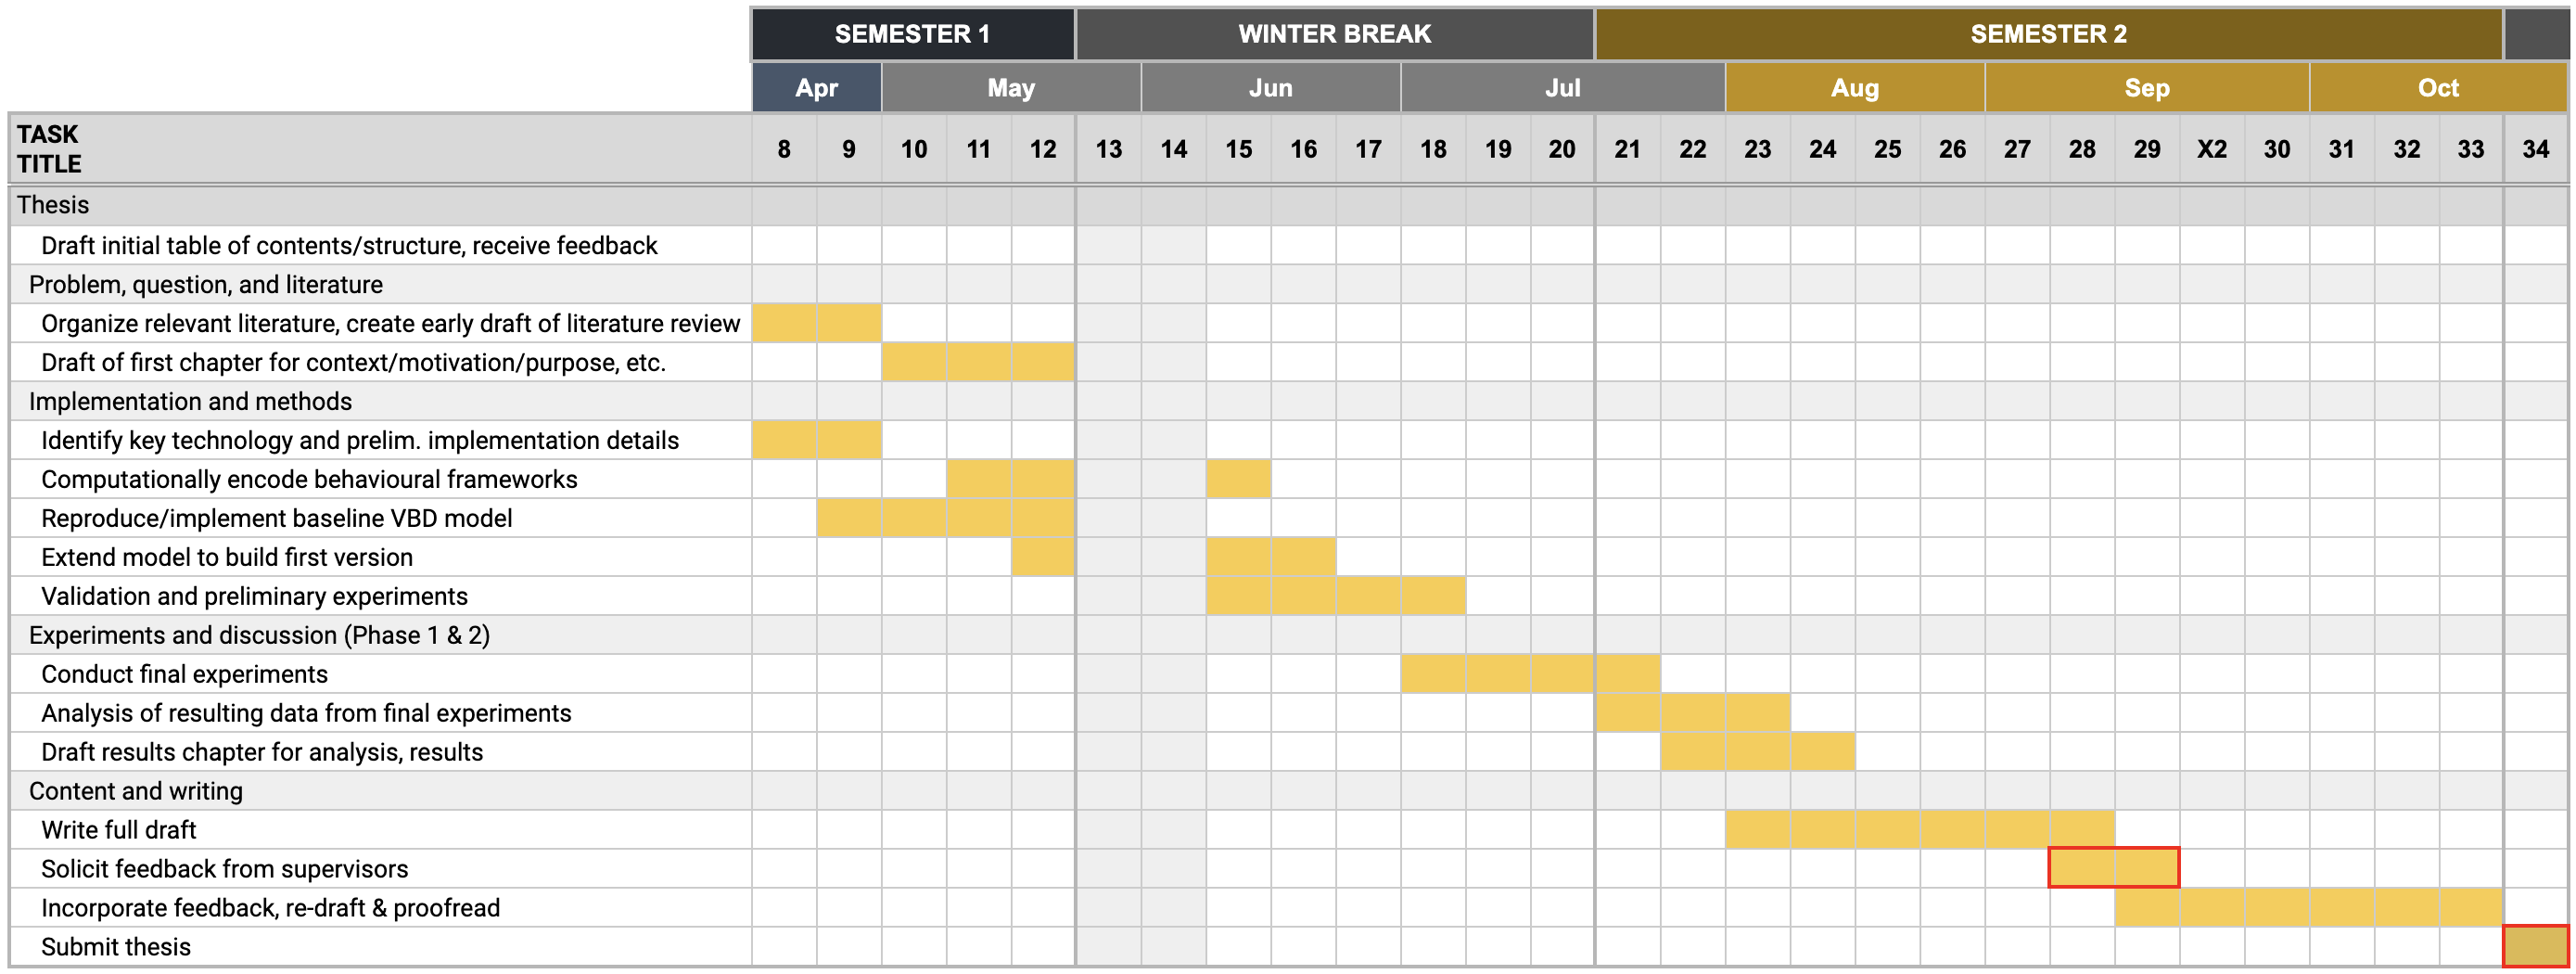
\includegraphics[scale=0.45,angle=90,origin=c]{figures/research_timeline.png}
\bcaption{Proposed timeline for the research project as a Gantt chart.}{Week numbering starts at proposal deadline (Week 8). \textit{X2} is mid-semester break. Cells outlined in red indicate deadlines.}
\label{fig:timeline}
\end{figure}
% \clearpage

\section{Expected contributions and implications}

This proposed research aims to contribute both a methodological contribution to the modelling community, and an investigation into a neglected area of research in the field of VBDs. The first phase of the project will contribute an extension of an existing ABM to develop a generic framework for modelling VBDs with preventive measures. Additionally, the project will be one of the first research efforts to encode the \mbox{COM-B} model in an ABM and examine the consequences of alternative psychological behavioural theories as part of agents' decision-making processes on VBD spread. The second phase of the project will illuminate characteristics of CBIs that effectively promote preventive behaviours within the ABM, and in turn, curb VBD spread.
\clearpage

% \bibliography{refs} % NOTE: this is my entire Zotero library.
\begin{singlespace}
\printbibliography[heading=bibintoc]
\end{singlespace}
\clearpage

%TC:ignore
\appendix
\appendixpage
\section{Baseline model description}\label{appendix:manore-abm}

In this appendix, I provide a brief description of the hybrid ABM for VBD spread from \citet{manore_network-patch_2015} for completeness. 


As described in Section~\ref{sec:baseline-model}, the dynamics for vector populations in the compartmental SEI model are given by the system of ODEs in \eqref{eq:mosquito}, where these equations represent a single population of vectors in patch $k$. It should be noted that each model of vector dynamics is patch-specific, though this is not denoted by any notation unless specified for emphasis. In the vector model, the rate of per-capita emergence, $h(N_v,t)$, the force of infection on vectors, $\lambda_v(t)$, and the force of infection on hosts, $\lambda_{h,j}(t)$, are comprised of various underlying parameters, which are described below.

The rate of per-capita vector emergence is defined as:

\begin{equation}
h(N_v,t)=N_v\left(\psi_v - \frac{r_v N_v}{K_v}\right)
\end{equation}

where $\psi_v$ is the natural per-capita emergence rate of vectors, $r_v=\psi_v-\mu_v$ is the intrinsic growth rate of vectors, and $K_v$ is the carrying capacity of vectors for the patch in question.

The force of infection on vectors is dependent on the rate of contact (biting) between hosts and vectors. This is an interaction that couples the ABM and EBM components of the hybrid model from \citet{manore_network-patch_2015}. To derive a force of infection on vectors, the number of bites between vectors and hosts is first calculated as:

\begin{equation}\label{eq:bites}
    b^{(k)}=\frac{\sigma_v N_v \sigma_h \hat{N}_h}{\sigma_v N_v + \sigma_h \hat{N}_h}
\end{equation}

where the superscript $(k)$ denotes the $k^{\text{th}}$ patch, $\sigma_v$ is the total number of bites a vector would yield if hosts were freely available, and $\sigma_h$ is the number of bites a host can sustain in a given time. Here, $\hat{N}_h=\sum_j{\alpha_j N^{(k)}_{h,j}}$ is the number of agents in the patch scaled by their exposure amount $\alpha_j$ according to their current activity $j$.

Naturally, the biting rates for hosts and vectors are derived from \eqref{eq:bites}. The number of bites per vector is given by $b^{(k)}_v=b^{(k)}/N_v$, and the average number of bites per host is given by $b_{h,j}^{(k)}=b^{(k)}/\hat{N}_h$. These biting rates are used to derive the force of infection on vectors and hosts based on the probability of disease transmission. The force of infection on vectors is given by:

\begin{equation}
    \lambda_v=b^{(k)}_v\cdot \beta_{vh}\cdot \left( \frac{\hat{I}_h}{\hat{N}_h} \right)
\end{equation}
where $\beta_{vh}$ is the probability of disease transmission from an infectious host to a vector, and $\hat{I}_h=\sum_j{\alpha_j I^{(k)}_{h,j}}$ is the scaled number of infectious hosts in the patch according to activity vector exposure. This value is used in the patch model \eqref{eq:mosquito}, coupling the patch and agent network models. The other direction of infection, from vector to host, is described by:

\begin{equation}
    \lambda_{h,j}=\alpha_jb^{(k)}_h\cdot \beta_{hv} \cdot \left(\frac{I_v}{N_v}\right)
\end{equation}
where $\beta_{hv}$ is the probability of disease transmission from an infectious vector to a host. Due to different exposure levels to vectors, the force of infection on hosts is specific to activities of agents, whereas the patch models of vectors encompass multiple activities.


As detailed in Section~\ref{sec:baseline-model}, the probabilities for progression through the agent SEIR disease states are transformations of agent-specific parameters, including $\lambda_{h,j}$. During each time step, agents progress from some disease state (S, E, or I) to another (E, I, or R) with some probability $p_j$. This is implemented in the ABM by the generation of a uniform random number $\theta\sim U[0,1]$, and the agent is progressed to the next disease state if $\theta < p_j$.

Table~\ref{table:manore-params} details the list of parameters used in the baseline model, and their interpretations.

\begin{table}[h]
    \centering
    \begin{adjustbox}{center}
        \footnotesize
        \begin{tabular}{cll} \toprule
            {Parameter} & {Description} & {Units} \\ \midrule
            $\psi_v$  & Per-capita emergence rate of vectors & vectors$/$time \\
            $\mu_v$  & Per-capita death rate of vectors  & vectors$/$time \\
            $K_v$  & Carrying capacity of vectors in the patch  & vectors \\
            $\sigma_v$  & Ideal number of bites a vector can carry out, if hosts were freely available  & bites$/$time \\
            $\sigma_h$  & Maximum number of bites a host can sustain in a given time period & bites$/$time \\
            $\beta_{vh}$  & Probability of disease transmission from an infectious host to a susceptible vector  & dimensionless \\
            $\beta_{hv}$  & Probability of disease transmission from an infectious vector to a susceptible host  & dimensionless \\
            $\nu_v$  & Rate of progression of vectors from the exposed (E) state to the infectious (I) state  & time$^{-1}$ \\
            $\nu_h$  & Rate of progression of hosts from the exposed (E) state to the infectious (I) state  & time$^{-1}$ \\
            $\gamma$ & Rate of recovery for hosts   & time$^{-1}$ \\ \bottomrule
        \end{tabular}
    \end{adjustbox}
    \bcaption{Parameters for the vector model.}{Adapted and expanded from \citet{manore_network-patch_2015}.}
    \label{table:manore-params}
\end{table}

%TC:endignore

\end{document}